%!TEX root = ../main.tex

\chapter{Experiments and Evaluations}
\label{chp:experiments}

What we have explained up to this chapter, model design and training, covers a relatively small part of the timeline of this study. We spent most of our time trying to understand the behavior of the produced models, collecting data about these behaviors, visualizing them, and comparing them with each other. 

The design and the implementation we have described up to this point refer to our base model, which is the model we used as the starting point and the reference for the other variants we produced with little adjustments and extra features. In this chapter, we will describe the other models we have developed. Next, we will select 4 top performers among them, and provide a more in-depth analysis regarding their behaviors and performances. Finally, we will talk about other experiments we conducted to explore our third-order model further.

\section{Data}
\label{sec:train_data}

Firstly, we will describe the data we use to train our model. We use a dataset called \verb|text8|, which was created by Matt Mahoney \cite{text8}. It is the first 100,000,000 bytes of plain text data obtained by truncating another file (\verb|fil9|, 715 MB) containing data from English Wikipedia \footnote{For details: \url{https://mattmahoney.net/dc/textdata.html}}. For ease of use, it is cleaned, meaning all the tables, links, citations, footnotes, and markups have been removed and hypertext links, numbers, and image captions are converted to ordinary text. The author describes the purpose of this dataset as a way to allow quicker testing, but we concluded this size of a corpus is sufficient and ideal considering the scope of our work and resources.

This dataset contains 17,005,207 tokens with 253,854 types. After the preprocessing (described in \ref{sec:preprocessing}), we are left with 8,448,361 tokens and 63,459 types. Then after the subsampling (described in \ref{sec:subsampling}), we have 3,428,264 tokens and 253,854 types. Finally, after the training/validation split (described in Section \ref{sec:val_split}), we have 3,085,438 tokens for the training, and 340,822 tokens for validating, using the same number of types.

\section{Model variants}
\label{sec:variants}
In addition to our base model, we have trained numerous other versions. We have kept the ones that yielded acceptable results for further analysis. By this, we are left with 26 versions of our model. In this section, we will briefly describe what is different in each version. Before we start, we should note that all of these models employ the same text preprocessing (See Section \ref{sec:preprocessing}), but they differ in what other processes they apply to the training data, training hyperparameters we choose for them, and the tricks they employ in their training loop.

For reference, here are some of the hyperparameters and tricks used in our base model:
\begin{itemize}
    \item Subsampling is enabled with a subsampling threshold of $1e-5$.
    \item Low context removal is disabled.
    \item Embedding vectors are in $300$ dimensions.
    \item Dynamic context windows with $L=4$.
    \item Negative training samples per each positive sample, i.e. parameter $k$, is set to $5$.
    \item The validation set is $10\%$ of the corpus.
    \item Each batch consists of $128$ target words. (\verb|batch_size| = $128$)
    \item We run the training for $6$ epochs.
    \item Our learning rate is $0.003$.
    \item We use \verb|Adam| optimizer with no learning rate scheduling.
    \item The weights of $\myscore{+}{w, u_1, u_2}$ and $\myscore{-}{w, u_1, u_3}$ are the same in the calculation of the overall loss.
    \item The loss function is constructed exactly like how it is described in Section \ref{sec:loss}.
\end{itemize}

Now when we describe other variants, we will only mention what is different, without going into any further detail. In the following numbered list, each item index corresponds to a version number.

\begin{enumerate}
    \item Corresponds to the base model.
    \item Learning rate is increased to $0.004$, with a decay coefficient of $0.85$.
    \item Context window size $L$ is adjusted to the number of occurrences of the word in the corpus, to assign every word in the training set a somewhat similar number of context words.
    \item Low context removal enabled with low context threshold of $100$.
    \item Subsampling threshold is increased to $1e-4$.
    \item In the loss function, instead of softplus, we use shifted \ac{ReLU} (Similar to SReLU in \cite{srelu}) with a shifting factor of $+1e-5$.
    \item Trying for a lucky initialization. Before we kick off the training loop, we try out $500$ random initializations and select the one with minimal loss for the training.
    \item Can a smaller batch size add to the ability of generalization? Batch size is lowered down to $64$.
    \item If we use a larger batch size to utilize our GPU resources better, how will it affect our model performance? To investigate this, the batch size is increased to $256$.
    \item Negative correction to the $\myscore{+}{w, u_1, u_2}$, for making sure if our implementation is correct.
    \item Replacing the softplus function in our loss with the Gaussian function\footnote{For details, see \url{https://en.wikipedia.org/wiki/Gaussian_function}}, followed by clamping the minimum to $1e-40$.
    \item Do the negative samples overpower the positive ones? Using a coefficient of $0.5$ for the $\myscore{-}{w, u_1, u_3}$ in the loss calculation.
    \item Using a coefficient of $0.2$ for the $\myscore{-}{w, u_1, u_3}$ in the loss calculation.
    \item Will regularization help us? Adding a dropout layer to the target and context embeddings. In other words, calculating loss using the embedding vectors with randomly disabled weights. The dropout rate is set to $0.4$ for both matrices.
    \item Applying dropout only to the target embeddings, again with the dropout rate of $0.4$.
    \item Using only $\myscore{+}{w, u_1, u_2}$.
    \item Deriving the calculation of $\myscore{-}{w, u_1, u_3}$ from the calculation of $\myscore{+}{w, u_1, u_2}$.
    \item Simplifying the loss function: Eliminating softplus from $\myscore{-}{w, u_1, u_3}$ and apply sigmoid directly to $D = P_\mathit{context} - P_\mathit{noise}$.
    \item Again eliminating softplus from $\myscore{-}{w, u_1, u_3}$, and replacing softplus with \ac{ReLU} in $\myscore{+}{w, u_1, u_2}$.
    \item Again eliminating softplus from $\myscore{-}{w, u_1, u_3}$, and replacing softplus with absolute function in $\myscore{+}{w, u_1, u_2}$.
    \item Rethinking our 3rd order loss: Conversion to the 2nd order with converging context projections to a $\delta$ value, and pushing the noise projections to the left. ($\delta = 5$)
    \item Same as the previous version, but this time $\delta$ is a random integer sampled from $[2,10]$ for each batch.
    \item Shifting weights for $\myscore{+}{w, u_1, u_2}$ and $\myscore{-}{w, u_1, u_3}$ in loss calculation. $w_p$ is the weight of $\myscore{+}{w, u_1, u_2}$, and $w_n$ is for $\myscore{-}{w, u_1, u_3}$. Training starts with the values $w_p = 0.92$, $w_n = 0.08$. It slowly shifts values until at the end of the training we reach $w_p = 0.5$, $w_n = 0.5$.
    \item Same as the previous one, but this time the values of $w_n$ and $w_p$ are switched.
    \item We again use weights for $\myscore{+}{w, u_1, u_2}$ and $\myscore{-}{w, u_1, u_3}$. But this time, we start by $w_p = 0.0$ and $w_n = 1.0$. Until the end of the training, these weights flip at every epoch.
    \item Eliminating $\myscore{+}{w, u_1, u_2}$ and only using the simplified version (only sigmoid, no softplus) of $\myscore{-}{w, u_1, u_3}$.
\end{enumerate}

We kept these models and eliminated some other versions because these were the ones that showed an acceptable performance and a reasonable learning curve in the training loop. Most of these models show similar performances, while the rest are slightly less impressive. It will be a waste of space and not be so useful to describe how every model performs and what their learning curves look like. Therefore we decided to pick the base model and a few other top performers and move on with this chapter using only them.


\section{Analysis of top four performers}

Now that we have shared the ideas we have experienced with, we can outline the behaviors and capabilities of these models. For this section, we decided to move with four models, namely, the \textbf{base model}, \textbf{version 15}, \textbf{version 18}, and \textbf{version 26}. We based our decision on the selection of these models to our immediate evaluations (see Section \ref{sec:immediate}), learning curves, and their scores on the word similarity task using the \verb|WordSim353| dataset. More about this dataset will be provided later in this section. As we mentioned earlier, a lot of our versions yield very similar performances. In those cases, we favored the models that were produced with more distinct ideas.

\subsection{Learning curves and immediate evaluations}
Before further analysis, we will first share how these models learned and how they performed in our immediate evaluations.

Table \ref{tab:loss_curves} shows the loss curves for all 4 models, throughout the 6 epochs.

\begin{table}[ht]
  \centering
  \begin{tabular}{cc}
    \begin{subfigure}{0.45\textwidth}
      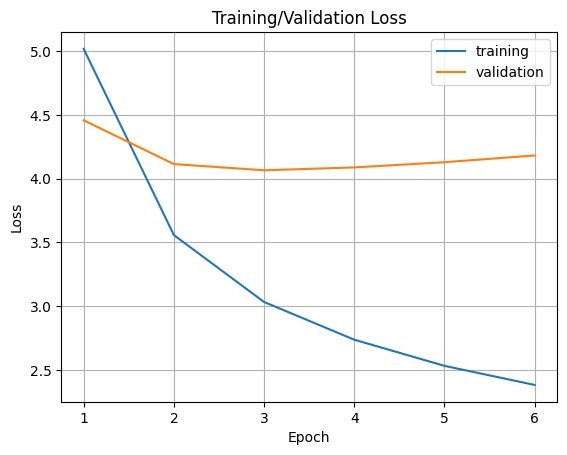
\includegraphics[width=\linewidth]{img/curve_base.png}
      \caption{Base Model}
    \end{subfigure} & 
    \begin{subfigure}{0.45\textwidth}
      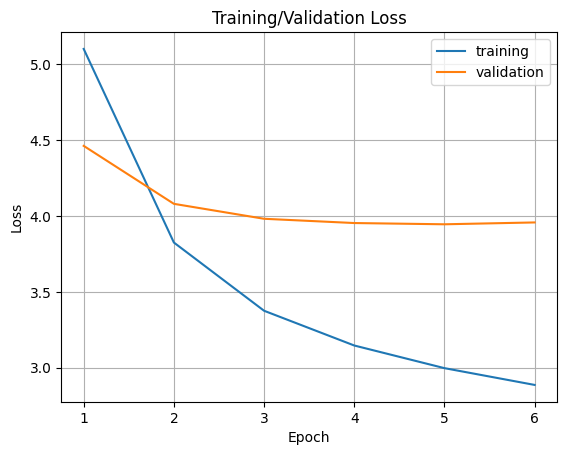
\includegraphics[width=\linewidth]{img/curve_15.png}
      \caption{Version 15}
    \end{subfigure} \\
    \begin{subfigure}{0.45\textwidth}
      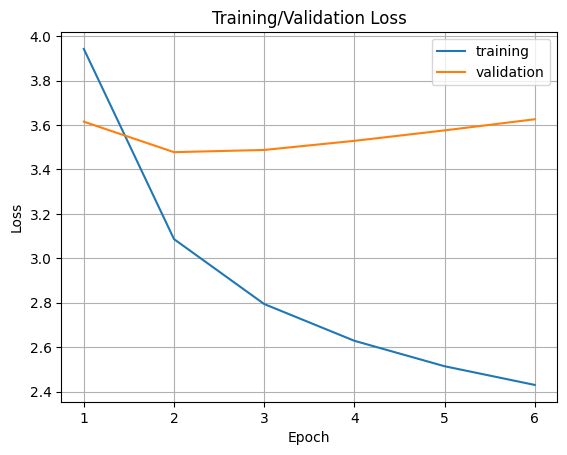
\includegraphics[width=\linewidth]{img/curve_18.png}
      \caption{Version 18}
    \end{subfigure} & 
    \begin{subfigure}{0.45\textwidth}
      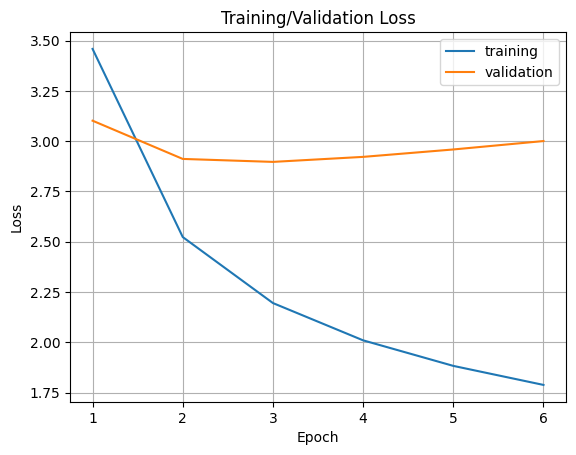
\includegraphics[width=\linewidth]{img/curve_26.png}
      \caption{Version 26}
    \end{subfigure}
  \end{tabular}
  \caption{Training and validation loss curves for each model}
  \label{tab:loss_curves}
\end{table}

We see that for all models, the loss of the training data keeps going down until the end. However, this is not the case for the validation loss. Except for version 15, we see no improvement, in contrast, we see a slight deterioration in the validation loss. This tells us that our model fits too well to the occurrences in the training partition in just a few epochs so that it fails to recognize how these words could have been positioned in any other piece of text outside of this data. This is a clear indication of overfitting. %However, we are hesitant to conclude the models are in a better state at the end of the third epoch, than how they are at the end of the training loop.

For the case of version 15, we see that regularization with the dropout layer adds up to the model's generalization abilities. We cannot complain about what the validation loss curve looks like by the end of 6 epochs.

As the differences between these models are mainly about the way they calculate their losses, the numerical values of losses are not directly comparable. The only meaningful comparison could be between the base model and the model version 15, which we see even though the base model has a better training loss, version 15 performs better on the validation data.

Now we show the performances of these models on our immediate evaluations (see Section \ref{sec:immediate}).

\begin{table}[ht]
  \centering
  \begin{tabular}{cc}
    \begin{subfigure}{0.45\textwidth}
      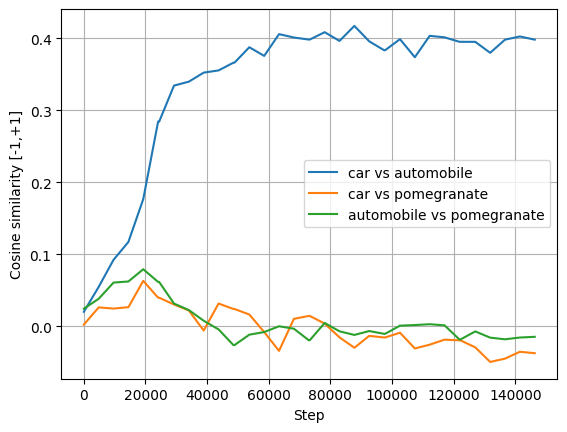
\includegraphics[width=\linewidth]{img/pom_base.png}
      \caption{Base Model}
    \end{subfigure} &
    \begin{subfigure}{0.45\textwidth}
      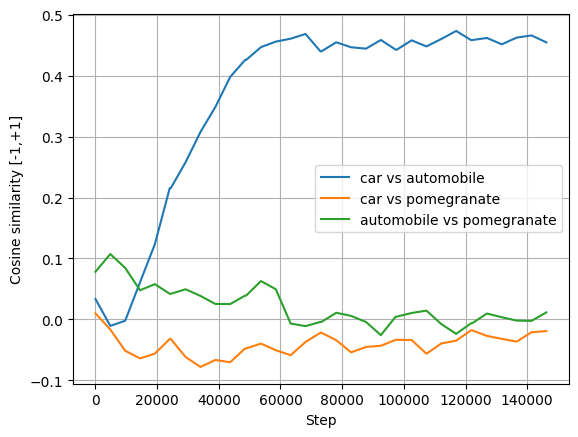
\includegraphics[width=\linewidth]{img/pom_v15.png}
      \caption{Version 15}
    \end{subfigure} \\
    \begin{subfigure}{0.45\textwidth}
      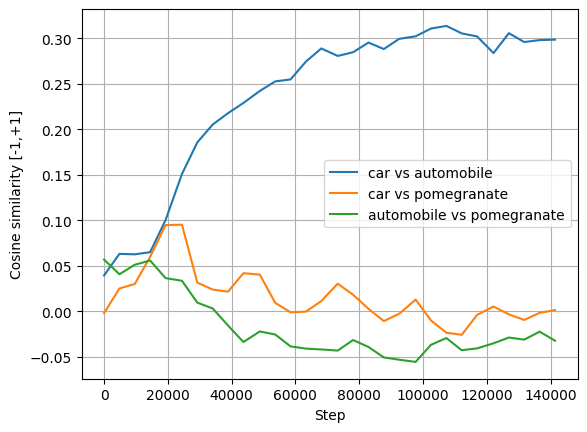
\includegraphics[width=\linewidth]{img/pom_v18.png}
      \caption{Version 18}
    \end{subfigure} &
    \begin{subfigure}{0.45\textwidth}
      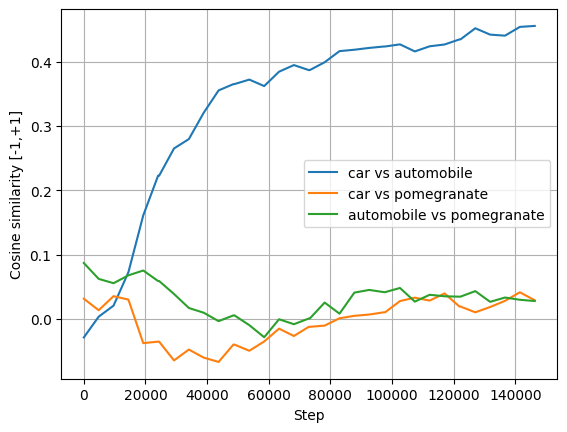
\includegraphics[width=\linewidth]{img/pom_v26.png}
      \caption{Version 26}
    \end{subfigure}
  \end{tabular}
  \caption{Cosine similarity-based immediate evaluations of models}
  \label{tab:pom_plots}
\end{table}

In Table \ref{tab:pom_plots}, we show how our models improve as they learn according to our cosine similarity-based evaluation. We see that each of these models can easily distinguish what should be similar and what should not from very early on, leaving a good impression before we move to large-scale similarity-based evaluations. Next, we share the closest neighbors to our test words, according to our selected models.

% BASE
\begin{table}[!ht]
\centering
\begin{tabular}{|c|c|c|c|c|}
\hline
\rowcolor[HTML]{330001} 
{\color[HTML]{FFFFFF} car} & {\color[HTML]{FFFFFF} money} & {\color[HTML]{FFFFFF} flower} & {\color[HTML]{FFFFFF} japan} & {\color[HTML]{FFFFFF} suspicious} \\ \hline \rowcolor[HTML]{E2EFDA} 
chevrolet & demand & perennials  & daigo & parchamis \\ \hline
cars & pricing & cultivation & taiwan & plebs  \\ \hline \rowcolor[HTML]{E2EFDA} 
motor & dividends  & sunflower & niigata & pdpa   \\ \hline
bmw & loans & hibiscus & korea & parcham \\ \hline \rowcolor[HTML]{E2EFDA} 
driver & profits & petals & meiji & negotiating \\ \hline
nhra & tax & sepals & prefecture & confidence \\ \hline \rowcolor[HTML]{E2EFDA} 
motors & repay & edible & japanese & khalq  \\ \hline
automobile & bonuses & flowers & takano & blamed \\ \hline \rowcolor[HTML]{E2EFDA} 
chassis  & cheques & shrubs & kitakyushu & advisers \\ \hline
\end{tabular}
\caption{Closest neighbors evaluation for the base model}
\label{tab:base-neighbors}
\end{table}

% V15
\begin{table}[!ht]
\centering
\begin{tabular}{|c|c|c|c|c|}
\hline
\rowcolor[HTML]{330001} 
{\color[HTML]{FFFFFF} car} & {\color[HTML]{FFFFFF} money} & {\color[HTML]{FFFFFF} flower} & {\color[HTML]{FFFFFF} japan} & {\color[HTML]{FFFFFF} suspicious} \\ \hline \rowcolor[HTML]{E2EFDA} 
mercedes & securities & pear & tokyo & qaida  \\ \hline
truck & profits & petals & honshu & told   \\ \hline \rowcolor[HTML]{E2EFDA} 
mans & gambling & foliage & japanese & campaign \\ \hline
coupe & wages & stalks & korea & corrupt \\ \hline \rowcolor[HTML]{E2EFDA} 
automobile & dollars & fruit & manchuria  & harshly \\ \hline 
cars & depositors & bees & china & resignations \\ \hline \rowcolor[HTML]{E2EFDA} 
chevrolet & exploitative & flowers & meiji & dissenters \\ \hline
daytona  & price & larvae & indonesia  & scorched \\ \hline \rowcolor[HTML]{E2EFDA} 
driver & repay & buckwheat & tokugawa & nationalists \\ \hline 
\end{tabular}
\caption{Closest neighbors evaluation for version 15}
\label{tab:v15-neighbors}
\end{table}

% V18
\begin{table}[!ht]
\centering
\begin{tabular}{|c|c|c|c|c|}
\hline
\rowcolor[HTML]{330001} 
\multicolumn{1}{|c|}{\cellcolor[HTML]{330001}{\color[HTML]{FFFFFF} car}} & \multicolumn{1}{c|}{\cellcolor[HTML]{330001}{\color[HTML]{FFFFFF} money}} & \multicolumn{1}{c|}{\cellcolor[HTML]{330001}{\color[HTML]{FFFFFF} flower}} & \multicolumn{1}{c|}{\cellcolor[HTML]{330001}{\color[HTML]{FFFFFF} japan}} & \multicolumn{1}{c|}{\cellcolor[HTML]{330001}{\color[HTML]{FFFFFF} suspicious}} \\ \hline
\rowcolor[HTML]{E2EFDA} 
mans & price & mentha & hirohito  & ilyas \\ \hline
driver & sell & corolla & kansai & detractors \\ \hline
\rowcolor[HTML]{E2EFDA} 
chassis  & prices & hibiscus & maldives & inappropriately \\ \hline 
engined  & spending  & shrubs & taiwan & justified \\ \hline
\rowcolor[HTML]{E2EFDA} 
cars & liquidity & kiwifruit & svalbard & tensions \\ \hline
miata & earnings  & snowmen & toshiki & alarmed \\ \hline
\rowcolor[HTML]{E2EFDA} 
benz & profit & laurel & dynasties & pledges  \\ \hline
mercedes & issuer  & leaf & nmt & assurances \\ \hline
\rowcolor[HTML]{E2EFDA} 
bmw & monetary & vines & korea  & accept \\ \hline
\end{tabular}
\caption{Closest neighbors evaluation for the version 18}
\label{tab:v18-neighbors}
\end{table}

%V26
\begin{table}[!ht]
\centering
\begin{tabular}{|c|c|c|c|c|}

\hline \rowcolor[HTML]{330001} 
\textcolor[HTML]{FFFFFF}{car} & \textcolor[HTML]{FFFFFF}{money} & \textcolor[HTML]{FFFFFF}{flower} & \textcolor[HTML]{FFFFFF}{japan} & \textcolor[HTML]{FFFFFF}{suspicious} \\ \hline \rowcolor[HTML]{E2EFDA} 

miata & loans & cucumber & nagano & shia \\ \hline
driver & taxes & stamens & hong & evocation \\ \hline \rowcolor[HTML]{E2EFDA} 
automobile & monetary & floral & singapore & azzam \\ \hline 
truck & borrow & foliage & china & leftist \\ \hline \rowcolor[HTML]{E2EFDA} 
crash & wages & petals & kyushu & denied \\ \hline
engined & fund & inflorescence & osaka & walid \\ \hline \rowcolor[HTML]{E2EFDA} 
cars & funds & sepals & japanese & refusing \\ \hline
chassis & earnings & hibiscus & meiji & entrenched \\ \hline \rowcolor[HTML]{E2EFDA} 
chevrolet & payments & strawberry & tokyo & shehri \\ \hline

\end{tabular}
\caption{Closest neighbors evaluation for the version 26}
\label{tab:v26-neighbors}
\end{table}


\subsection{Statistics: Performance and characteristics}
\label{sec:stats}

We believe that the best way to understand the behavior of our models is to observe how they organize the vectors in the vector space, and how these behaviors change as they learn. For this purpose, we gathered the models we saved at the end of each epoch, computed some statistics, and tried to see if we could find any useful trend embedded in these numbers.

To keep a balance between computational efficiency and the fair representation of the vector space, we sampled a subset of words from our vocabulary to conduct our computations.

\begin{figure}[ht]
    \centering
    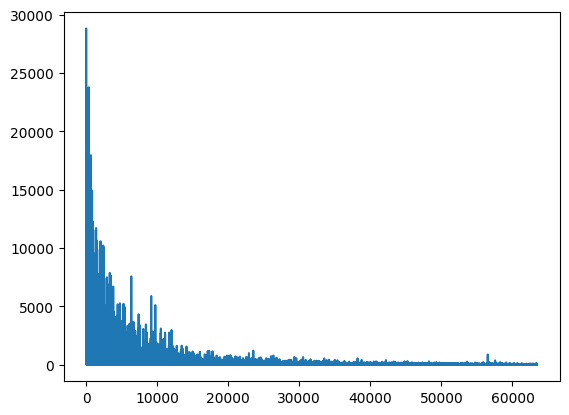
\includegraphics[width=0.7\textwidth]{img/word_counts.png}
    \caption{Word frequencies in our training corpus.}
    \label{fig:word_counts}
\end{figure}

Figure \ref{fig:word_counts} shows the frequencies of the types in our vocabulary in the corpus, partially sorted from the most frequent to the least. We decided that instead of sampling $n$ words from anywhere in the corpus, it would be more logical to select a frequency range that represents the average case and sample our test words from there. Following this, we sampled $50$ words from the set of words that appear in our corpus $f$ times, where $f \in [100, 20000]$. 5 of these test words are:

\begin{displayquote}
\centering
'televised', 'uruguayan', 'credits', 'geologist', 'commerce'
\end{displayquote}

Next, for all of our test words, we collected all the words that appear in their context windows and also sampled some noise words. Then for each test word, we picked the 100 most frequent context words and the 100 most frequent noise words and eliminated the rest. Now that we have our target words, combined with their context and noise samples, we are ready to proceed to our computations.

We have selected 6 statistics that we believe can give us useful insights and expose some interesting patterns. These 6 statistics are:

\begin{enumerate}
    \item Average context word (context representation) projections onto the target word (target representation).
    \item Average noise word (context representation) projections onto the target word (target representation).
    \item Average \textbf{variance} of the context words (context representation) projections onto the target word (target representation).
    \item Average projection \textbf{difference} of the context words (context representation) and the noise words (context representation) onto the target word (target representation).
    \item Average \textbf{cosine similarity} of a context word (target representation) and the target word (target representation).
    \item Average target word (target representation) magnitude.
\end{enumerate}

For each model, we calculated these statistics, for all of its models produced at the end of each 6 epochs. Also to give a better view, we conducted the same calculations for a random model, you will see it as "Epoch 0" in the plots. All the statistics listed above are visualized for our selected four models in Figure \ref{fig:stats_base}, Figure \ref{fig:stats_v15}, Figure \ref{fig:stats_v18}, and Figure \ref{fig:stats_v26}, for the base model, version 15, version 18, and version 26, respectively. You will notice that the plots are designed to show how these metrics change starting from the random initialization to the final epoch. The numbers used in the labels correspond to the indexes used in the above list. 

\begin{figure}[!ht]
    \centering
    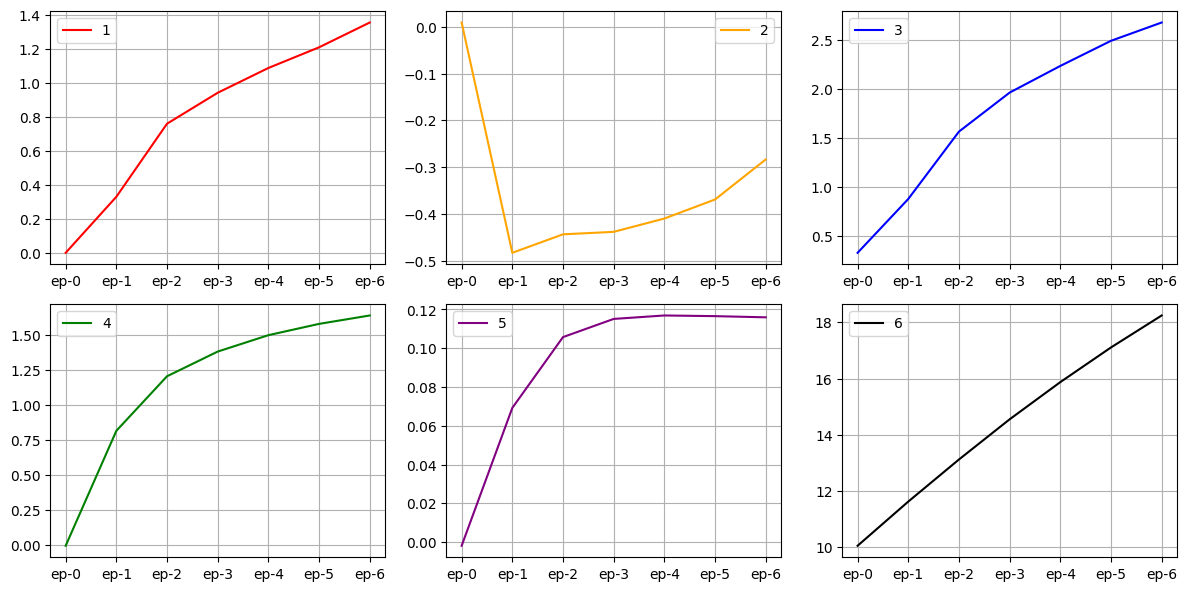
\includegraphics[width=1.0\textwidth]{img/stats_base.png}
    \caption{Statistics for the base model}
    \label{fig:stats_base}
\end{figure}

\begin{figure}[!ht]
    \centering
    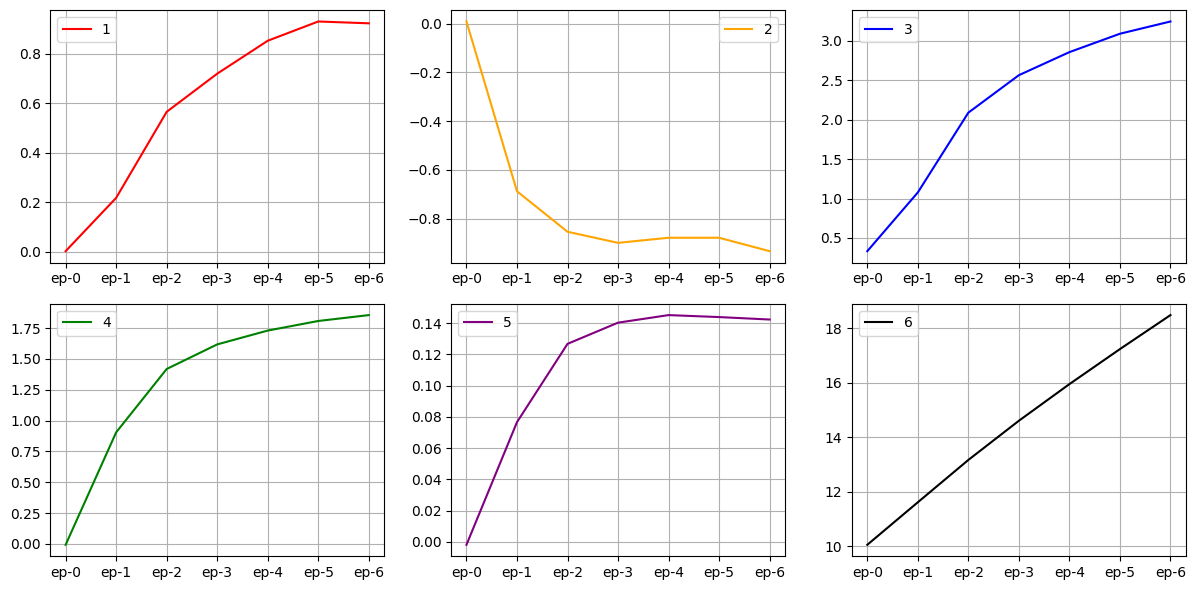
\includegraphics[width=1.0\textwidth]{img/stats_v15.png}
    \caption{Statistics for version 15}
    \label{fig:stats_v15}
\end{figure}

\begin{figure}[!ht]
    \centering
    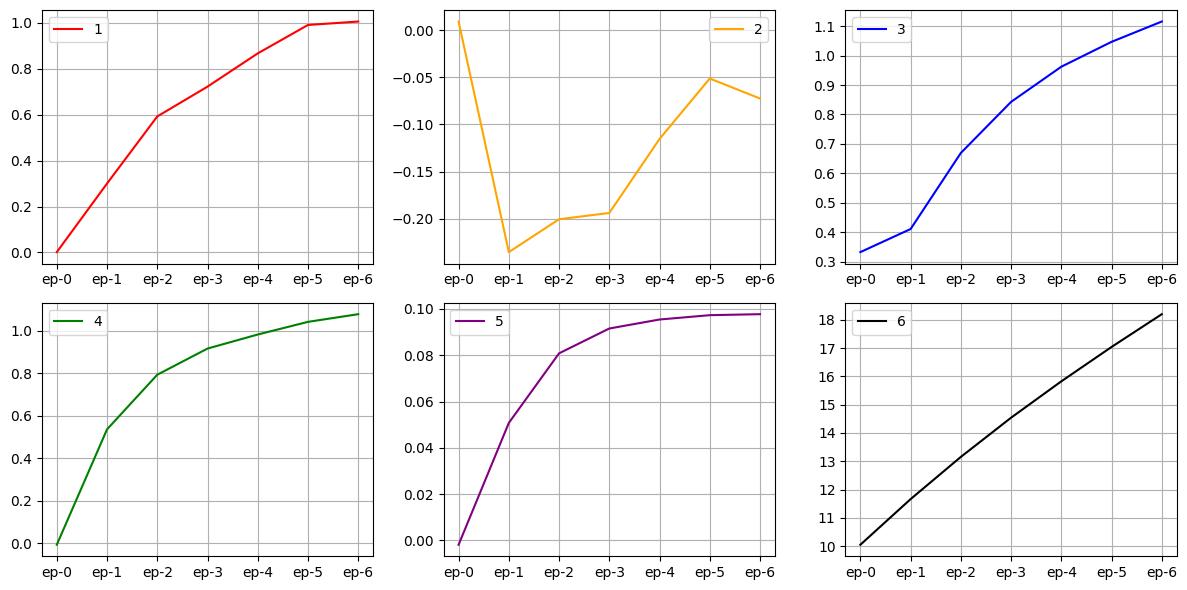
\includegraphics[width=1.0\textwidth]{img/stats_v18.png}
    \caption{Statistics for version 18}
    \label{fig:stats_v18}
\end{figure}

\begin{figure}[!ht]
    \centering
    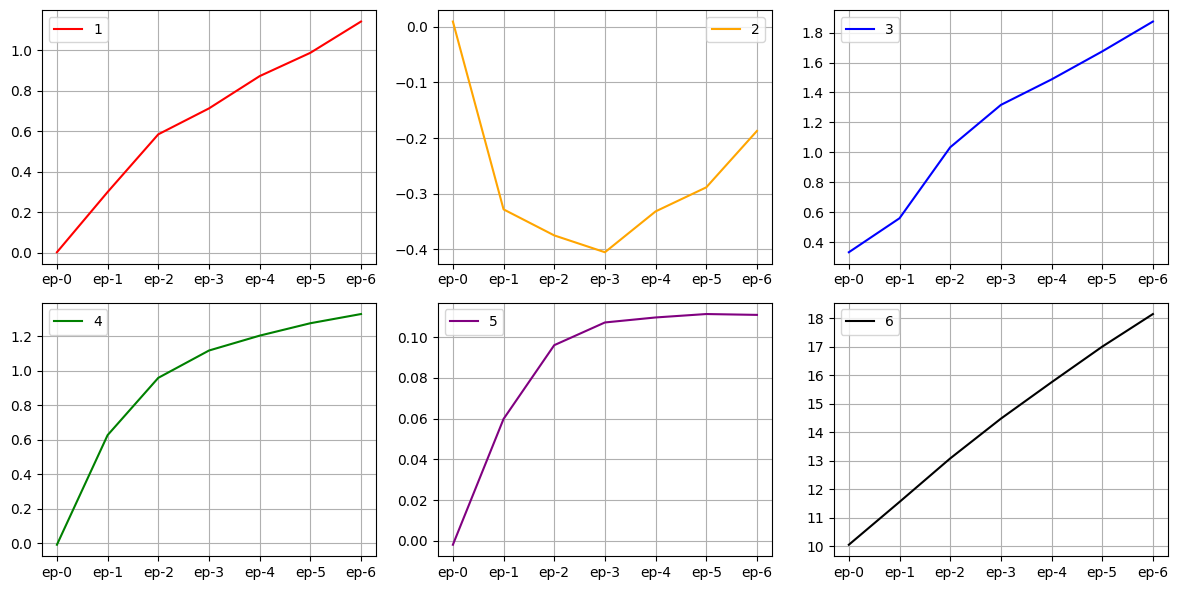
\includegraphics[width=1.0\textwidth]{img/stats_v26.png}
    \caption{Statistics for version 26}
    \label{fig:stats_v26}
\end{figure}


To commentate on what we see in these figures, the first thing we notice is that the trends followed by each model for every metric are somewhat similar to each other. For instance, we see that the statistic \#1 for each model goes up as the learning progresses. On the other hand, we see that statistic \#2 tends to go down with the learning, but for some models, it starts to go up after some point. We observe this increasing trend for all the models except for version 15. Oddly enough, version 15 is the only model in which we did not observe an increasing trend in its validation loss curve, which makes us think that these two observations are correlated.

Another thing we notice is that for all models, the variances of the context projections go up as the learning progresses. We are not able to interpret this with full confidence, because this might indicate several things. For one, which is the favored case, this might mean that we are creating context hyperplanes, and these groups of projections are becoming more and more distanced from each other. Another possibility is that our context projections are getting spread over the target vector, following no particular rule or trend.

We also see that our loss function, regardless of the version, makes our target vectors longer and longer, with a stable pace. 

Finally, the thing that we are glad to see the most is statistic \#4, which tells us that our loss function successfully pushes the noise projections to the left side of the context projections. Plus, this increase in projection difference keeps going up even when statistic \#2 starts following an increasing trend. 


\subsection{Visualizing vector projections}
\label{sec:vis_proj}

We now visualize the vector projections of the context and the noise words onto the target vectors of our test words. We randomly chose 20 target words from our test words for this task and calculated the orthogonal projections of the context vectors of the context and the noise words for each epoch. This will enable us to demonstrate how the vector space is organized as the model learns better about the training data.

For the sake of simplicity of our demonstration, we will share the projections of 3 target words instead of 20. In the following plots, you will find a bunch of green and red dots stacked together on different rows. Green dots represent the context projections, and the red dots represent the noise projections. Each dot from both colors represents an orthogonal projection of a context vector (context word or a noise word) onto the target vector. Context vector projections are stacked in a way so that the bottom row corresponds to the initialization and the topmost row corresponds to the last epoch. For the noise projections, it is the opposite, with the topmost row corresponding to the initialization and downward proceeding with the next epoch until the bottom-most. 

The blue lines in the middle of the figures represent the target vector. We can see which target are we looking at from the label placed on the top right corner of each figure. The numbers on the left side of the figures have no meaning. In addition, the black dots placed towards the middle of the group in each row show where the average of that row falls. For lines showing the same epochs, lines were drawn to describe the relative positions of the averages between the corresponding context and noise lines. 

\begin{table}[p]
  \centering
  \begin{tabular}{cc}
    \begin{subfigure}{0.95\textwidth}
      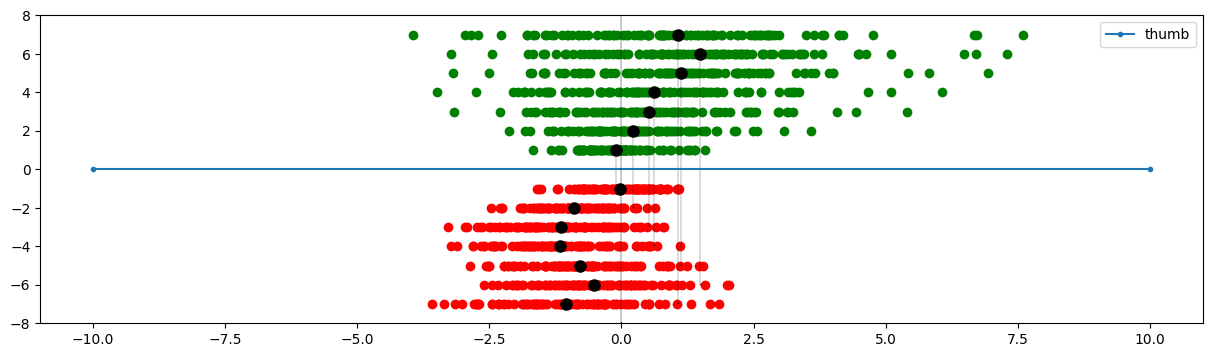
\includegraphics[width=\linewidth]{img/thumb_base.png}
      \caption{Target word: Thumb}
    \end{subfigure} \\
    \begin{subfigure}{0.95\textwidth}
      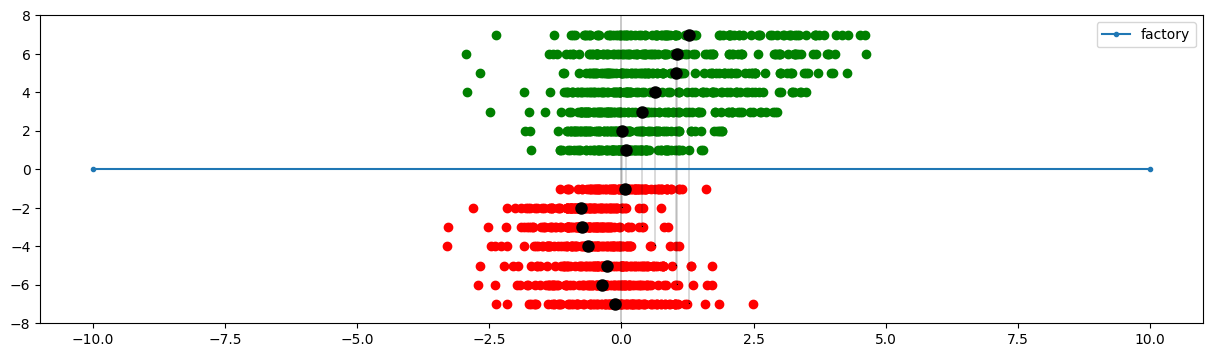
\includegraphics[width=\linewidth]{img/factory_base.png}
      \caption{Target word: Factory}
    \end{subfigure} \\
    \begin{subfigure}{0.95\textwidth}
      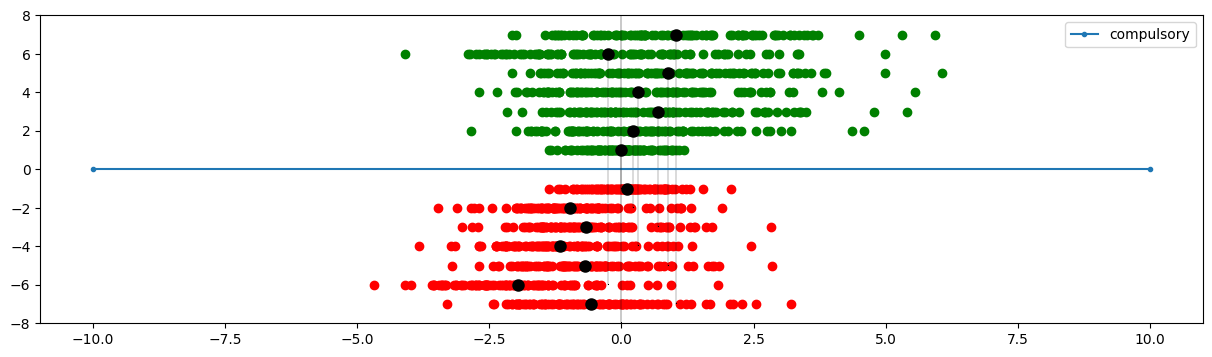
\includegraphics[width=\linewidth]{img/compulsory_base.png}
      \caption{Target word: Compulsory}
    \end{subfigure} 
  \end{tabular}
  \caption{Context and noise projections onto the target vector - Base Model}
  \label{tab:base_projections}
\end{table}


\begin{table}[p]
  \centering
  \begin{tabular}{cc}
    \begin{subfigure}{0.95\textwidth}
      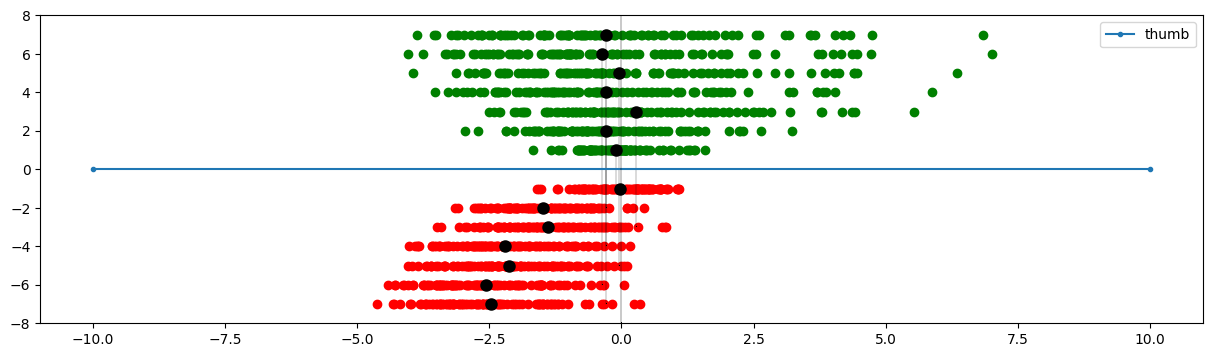
\includegraphics[width=\linewidth]{img/thumb_v15.png}
      \caption{Target word: Thumb}
    \end{subfigure} \\
    \begin{subfigure}{0.95\textwidth}
      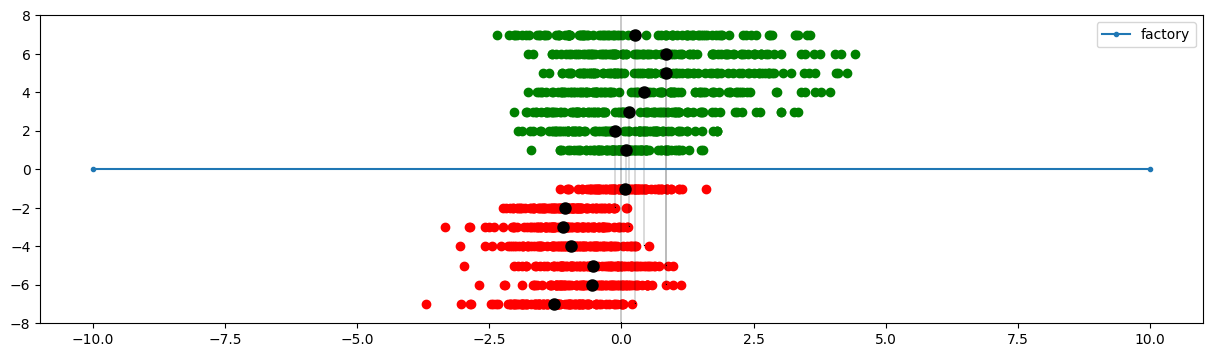
\includegraphics[width=\linewidth]{img/factory_v15.png}
      \caption{Target word: Factory}
    \end{subfigure} \\
    \begin{subfigure}{0.95\textwidth}
      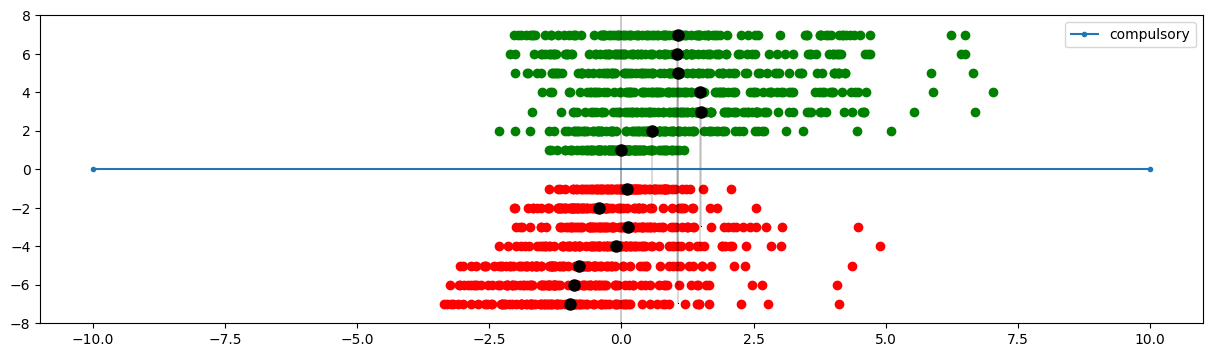
\includegraphics[width=\linewidth]{img/compulsory_v15.png}
      \caption{Target word: Compulsory}
    \end{subfigure} 
  \end{tabular}
  \caption{Context and noise projections onto the target vector - Version 15}
  \label{tab:v15_projections}
\end{table}


\begin{table}[p]
  \centering
  \begin{tabular}{cc}
    \begin{subfigure}{0.95\textwidth}
      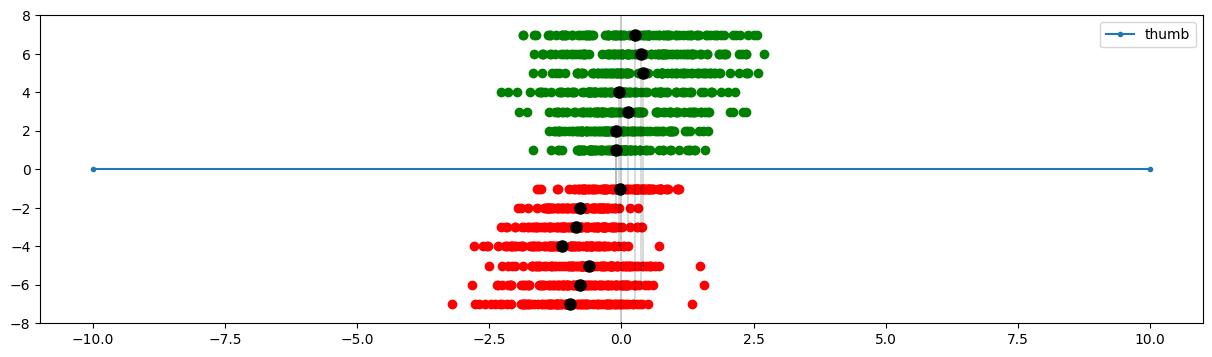
\includegraphics[width=\linewidth]{img/thumb_v18.png}
      \caption{Target word: Thumb}
    \end{subfigure} \\
    \begin{subfigure}{0.95\textwidth}
      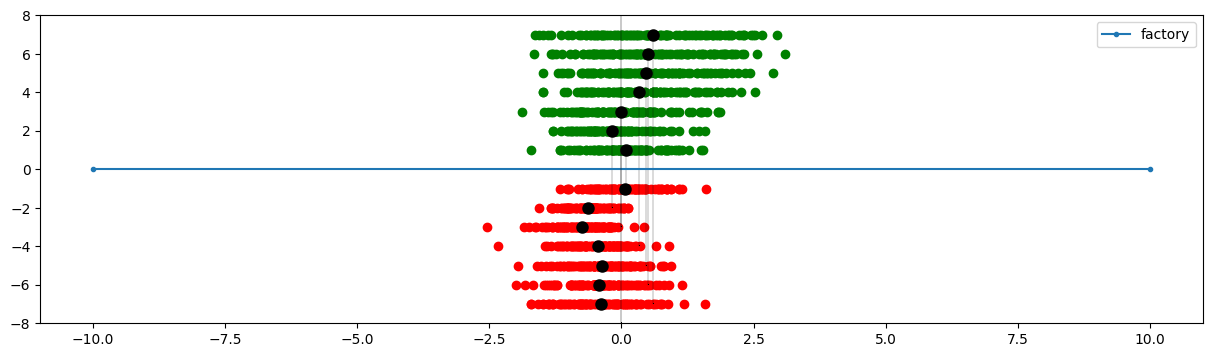
\includegraphics[width=\linewidth]{img/factory_v18.png}
      \caption{Target word: Factory}
    \end{subfigure} \\
    \begin{subfigure}{0.95\textwidth}
      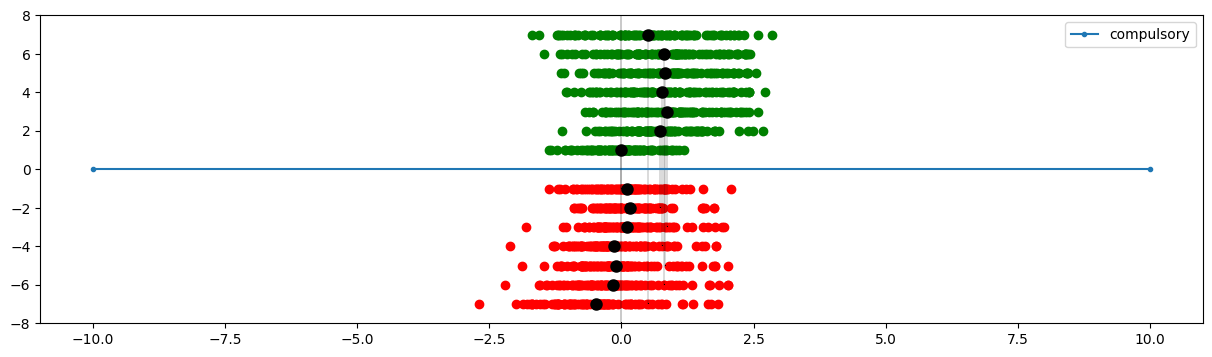
\includegraphics[width=\linewidth]{img/compulsory_v18.png}
      \caption{Target word: Compulsory}
    \end{subfigure} 
  \end{tabular}
  \caption{Context and noise projections onto the target vector - Version 18}
  \label{tab:v18_projections}
\end{table}


\begin{table}[p]
  \centering
  \begin{tabular}{cc}
    \begin{subfigure}{0.95\textwidth}
      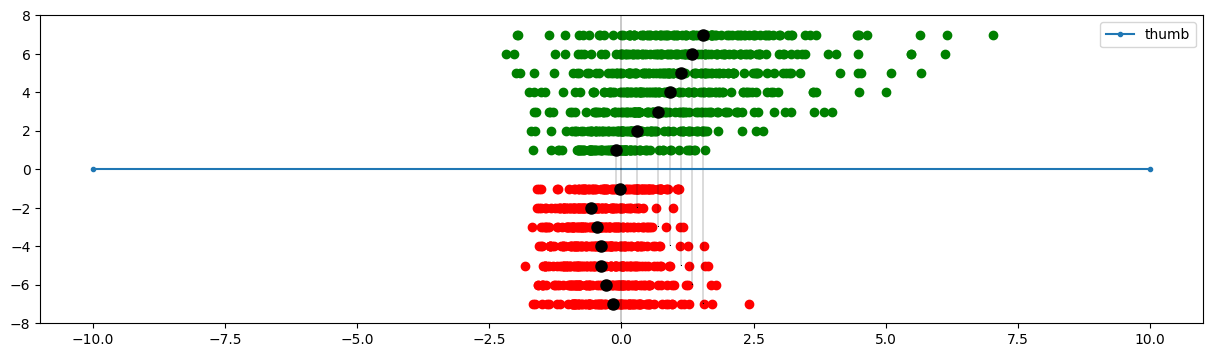
\includegraphics[width=\linewidth]{img/thumb_v26.png}
      \caption{Target word: Thumb}
    \end{subfigure} \\
    \begin{subfigure}{0.95\textwidth}
      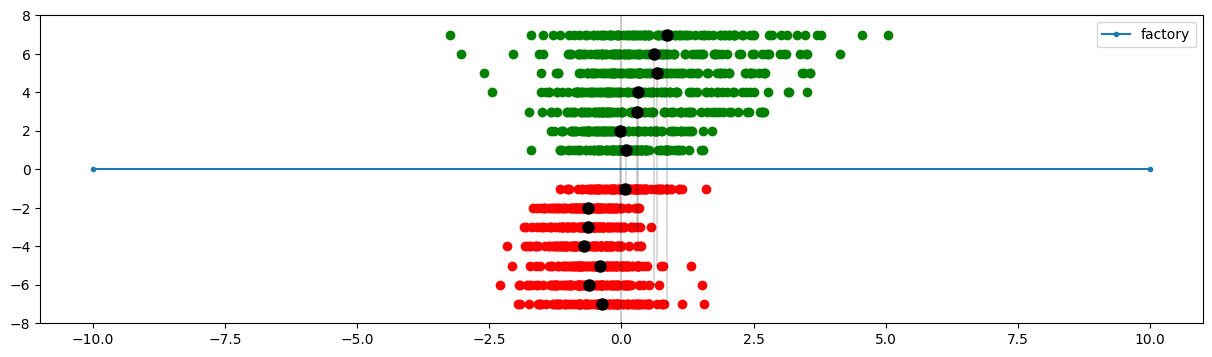
\includegraphics[width=\linewidth]{img/factory_v26.png}
      \caption{Target word: Factory}
    \end{subfigure} \\
    \begin{subfigure}{0.95\textwidth}
      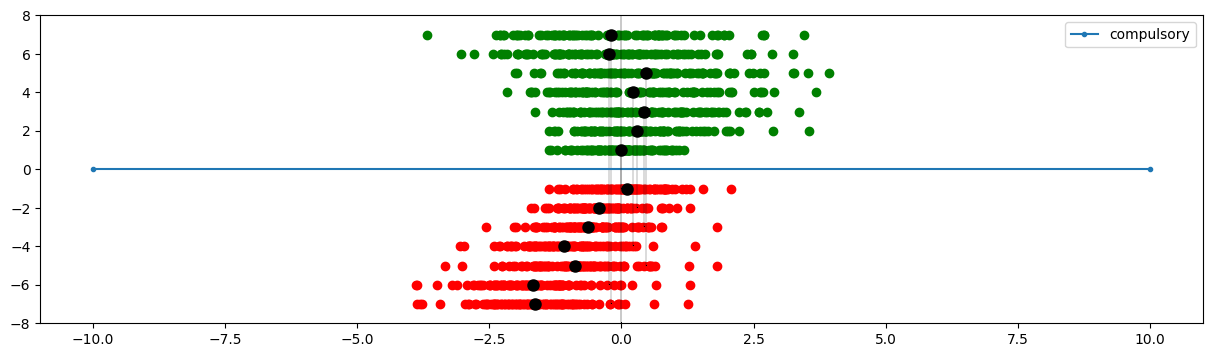
\includegraphics[width=\linewidth]{img/compulsory_v26.png}
      \caption{Target word: Compulsory}
    \end{subfigure} 
  \end{tabular}
  \caption{Context and noise projections onto the target vector - Version 26}
  \label{tab:v26_projections}
\end{table}

For three target words, "\textit{Thumb}", "\textit{Factory}" and "\textit{Compulsory}", we show the projections for each model in Table \ref{tab:base_projections}, Table \ref{tab:v15_projections}, Table \ref{tab:v18_projections}, and Table \ref{tab:v26_projections}.

Just like what we observed in the charts we presented earlier, we see that regardless of the shifting of the noise and context projections, the difference between them is always kept positive, and usually increases as epochs progress. It is interesting to see that sometimes we see noise word projections go right, or the context word projections go left, even though this is expected to diverge our loss. Nevertheless, even by doing this, seems like our models find the configuration that minimizes the loss better than the epoch before.

We see that the projections, especially the context word projections, get more and more spread with the learning. We fail to observe any obvious grouping of projections, which we believe would indicate the existence of context hyperplanes. 

We should note, however, that there is a possibility that a context word can be sampled also as a noise word in some of these plots. It is not very likely but we do not know for sure, and this can be the reason for outliers in some cases.

\subsection{Context word projections clustering}

% Maybe add a reference here
Aiming to find a hint of the existence of context hyperplanes, now we apply the k-means clustering algorithm to the context word projections. For all 50 test words and their context words we collected from our corpus, we calculate the context word projections onto the target embeddings of the test words. Then for each test word, we run the clustering algorithm on these projections. The k-means algorithm requires the number of clusters $k$ to be given beforehand. We run the clustering algorithm for different $k$ values, ranging between two and eight. This operation we described is conducted for all four models and each of their epochs.

We judge the quality of clusters given the values and $k$ using a metric called "\textit{Silhouette Score}". It is a metric that evaluates the compactness of the formed clusters, and the separation amongst them. From another perspective, it considers the similarity of an object to its cluster, compared to other clusters. This metric ranges between $[-1, 1]$, where $1$ is the most ideal clustering and $-1$ is the worst case.

For a single sample, let $a$ be the average intra-cluster distance and $b$ be the average nearest-cluster (except the cluster that the sample is assigned to) distance. The Silhouette Coefficient for a sample $s(i)$ is calculated as:

\[
s(i) = \frac{(b - a)}{\max(a, b)}
\]

The overall Silhouette Score $S$, which we use as the clustering score, is calculated as:

\[
S = \frac{\sum_{i \in P} s(i)}{|P|}
\]
\noindent
where $P$ is the full set of context projection values.

We calculated this score for each test word and for each epoch of each model. As the distribution of the projections is completely different for each word and in each model, it is not logical to calculate an average value among all test words. However, when we look at the clustering scores for each particular test word and model combination, we fail to see a clear clustering for any given $k$. Whatever is the $k$ value, we keep observing clustering scores ranging between 0.5 and 0.65, indicating that none of these $k$ values provide a clear grouping of these projection values. This means that we fail to prove the existence of context hyperplanes using a clustering approach.

We will omit the full list of results, but we share the scores for the test word "\textit{title}" for the final epochs of each model, in Table \ref{tab:title-clusters}. We observe similar results for every other case as well.

\begin{table}
\centering
\begin{tabular}{|c|c|c|c|c|}
\hline
\rowcolor[HTML]{330001} 
\cellcolor[HTML]{FFFFFF}{\color[HTML]{FFFFFF} }                 & {\color[HTML]{FFFFFF} base (Ep. 6)} & {\color[HTML]{FFFFFF} v15 (Ep. 6)} & {\color[HTML]{FFFFFF} v18 (Ep. 6)} & {\color[HTML]{FFFFFF} v26 (Ep. 6)} \\ \hline
\rowcolor[HTML]{FFFFFF} 
\cellcolor[HTML]{330001}{\color[HTML]{FFFFFF} Best k}           & 8                                     & 2                                    & 7                                    & 2                                    \\ \hline
\rowcolor[HTML]{FFFFFF} 
\cellcolor[HTML]{330001}{\color[HTML]{FFFFFF} Clustering Score} & 0.575                                 & 0.600                                & 0.597                                & 0.568                                \\ \hline
\end{tabular}
\caption{Clustering of context projections for the test word "title"}
\label{tab:title-clusters}
\end{table}


\subsection{Visualizing context projections}

Just to see what happens, now we employ a different approach and visualize the context projections, rather than the context word projections. The difference is that instead of visualizing the projections of each context word, we now calculate an average projection of each context of a test word and show that instead. A "context" of a word is the set of tokens that appear in the context window for one occurrence of that word. To be clearer, the projection of a context $c$ is:

\[
P(c) = \frac{\sum_{w \in c} p(w)}{|c|}
\]
\noindent
where $P(c)$ is the projection of the context $c$ and $p(w)$ is the projection of the context representation of the word $w$ onto the target representation of the target word.

\begin{table}[p]
  \centering
  \begin{tabular}{cc}
    \begin{subfigure}{0.95\textwidth}
      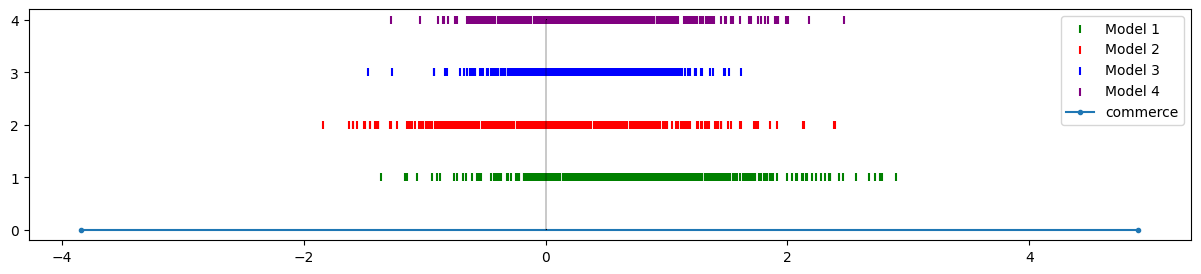
\includegraphics[width=\linewidth]{img/context_commerce.png}
      \caption{Target word: Commerce}
    \end{subfigure} \\
    \begin{subfigure}{0.95\textwidth}
      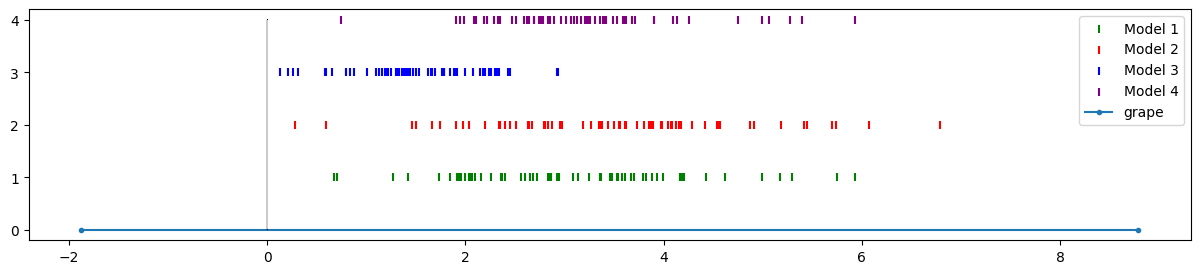
\includegraphics[width=\linewidth]{img/context_grape.png}
      \caption{Target word: Grape}
    \end{subfigure} \\
    \begin{subfigure}{0.95\textwidth}
      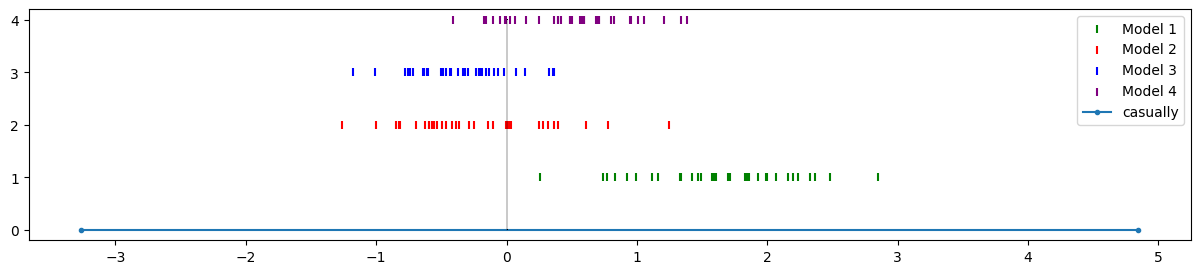
\includegraphics[width=\linewidth]{img/context_casually.png}
      \caption{Target word: Casually}
    \end{subfigure}
  \end{tabular}
  \caption{Context projections onto the selected target words, for the final models of all versions}
  \label{tab:context_proj}
\end{table}

We show the results for the final models of each version, using 3 test words, in Table \ref{tab:context_proj}. We pick the words "\textit{commerce}", "\textit{grape}", and "\textit{casually}". In the figures, we use the names "Model 1", "Model 2", "Model 3" and "Model 4", for the base model, version 15, version 18, and version 26, respectively. Even though it now seems like a projection grouping is relatively more distinguishable, we still fail to point out distinct clusters. 

\section{Comparative evaluations of top four performers}

Now we put our models head to head with some other well-known models pre-trained on very large corpora. We test our models on popular evaluation tests and use standardized evaluation datasets for it. We compare and visualize the results. By the end of this section, we will have a better understanding of the abilities and potentials of our 3rd-order model idea, compared to what is commonly considered "good" in the literature.

\subsection{Tasks and datasets}
\label{sec:tasks_datasets}

To evaluate the abilities of our models from different perspectives, we have chosen three different tasks to perform and several datasets for these tasks as standards. First, we conduct our evaluations in similarity and relatedness tasks, measuring for a given pair of words, how is the level of similarity calculated using our models compared to human judgment. Then we move to word analogy, where the semantic relationships of words are modeled in higher order, and we see if our models are fit for capturing these relationships. Finally, we designed a new evaluation, in which we check if our models are actually able to distinguish different word senses for the same word, given their contexts. This is a new task performed even for the standard models, we produce a new dataset for it and measure the scores achieved by both our models and the standard ones.

\subsubsection{Spearman's Rank Correlation Coefficient}

Before we go any further, we should first introduce the \textit{Spearman Correlation}. Named after its creator Charles Spearman, the Spearman correlation is a popular method for measuring how well the relationship between two variables can be described, using a monotonic function. It is related to but differs from its premise, the Pearson correlation, which examines linear relationships. The Spearman correlation is non-parametric, making it a better choice for variables with non-linear associations. By ranking the data, Spearman correlation measures the degree to which one variable's values change concerning another variable's values. It is a very handy tool for exposing underlying patterns and relations within the dataset. 

The Spearman correlation $\rho$ is calculated by first ranking the values of the two variables and then applying the following formula:

\[
\rho = 1 - \frac{6\sum d_i^2}{n(n^2 - 1)}
\]
\noindent
where $n$ is the number of data points and $d_i$ is the difference between the ranks of corresponding values in the two variables. The result ranges from in $[-1, 1]$, where $-1$ indicates an inverse relationship, $0$ represents no linear relationship, and $1$ implies a perfect direct relationship between the variables.

\subsubsection{Similarity and relatedness}

In this type of evaluation, we take as a reference a dataset containing a set of word pairs, and similarity (or relatedness) scores assigned to them by human annotators. Depending on the dataset, these scores are distributed in different ranges, such as $[0, 10]$, or $[0, 4]$. The similarity score tells us how similar are the meanings of two words, while relatedness measures the relatedness of these two meanings. For example, the words "\textit{car}" and "\textit{bus}" can be considered similar, given that both are the names of some sort of vehicle. On the other hand, the words "\textit{car}", "\textit{bus}" and "\textit{road}" are considered related, considering that they refer to related concepts. In essence, similarity is about the "is a" relation, meanwhile, relatedness is a more general concept, and can be expressed with an "is about" relation. Some datasets draw strict lines between these two terms, awarding one relation and penalizing the other.

This type of evaluation is perhaps the most standardized way of assessing the word representations intrinsically, probably because of the ease of computation, rapidness of implementation, and large community support with a variety of existing human-annotated similarity datasets. Also, considering that it is the method that one is most likely to find in any word embedding model publication, it provides a valuable benchmark to understand how a new model ranks amongst others. However, it definitely comes with its weaknesses, and we find them investigated thoroughly in the article \cite{sim-problems} where the authors analyze when and why this technique may yield unreliable and perhaps meaningless results. We now list what are some of the shortcomings of this approach and briefly mention their reasons. 

\begin{itemize}
    \item Human annotations of word similarity standards are subjective, and this is apparent even though most of the standardized datasets rely on recruiting of large group of annotators to cope with it.
    \item The majority of word embedding models presented are selected among their variants considering their performance on this task. But one should note that the selected model can be implicitly overfitting the used standard, and might fail in any other. 
    \item Even though we have implementation tricks to deal with this effect, we still cannot deny that word embedding models are sensitive to word frequencies in the training corpus. This will definitely impact how a model performs on over and underrepresented words in the evaluation set. In this case, it will be hard to defend that the obtained accuracy will reflect the true quality of the training mechanism and the produced embeddings.
    \item As described in \cite{sim-problems2}, word similarity-based judgments of embeddings rarely correlate with how well they serve their function in downstream \ac{NLP} tasks, such as text classification, parsing, and sentiment analysis.
\end{itemize}

We keep these in mind but still value this technique as a good indicator of how well a word embedding model learns about word semantics. We assess our vectors using this method, but also pair it with other sorts of assessments.

We followed the mechanism introduced in \cite{glove}, and built a testing mechanism similar to theirs. What we do is, for each word pair contained in the dataset, we calculate the cosine similarity using the vectors in hand, put the values for all pairs in a single list, and calculate Spearman's rank correlation coefficient of this list and the human scores provided in that dataset. We omit a word pair if at least one of the two words is not represented by the embedding model. This way, we understand how well our model ranks the similarities of these pairs in a similar way as the human annotators do.

We again consulted \cite{glove} to find out what are the common standards used for this purpose. In the end, we picked 3 of the datasets mentioned in this paper, and additionally find one ourselves. These datasets and their brief descriptions are provided in the following.

\begin{itemize}
    \item \verb|WordSim-353|: It is a quite popular similarity and relatedness benchmark, containing 353 samples annotated by human annotators \cite{wordsim}. The dataset contains annotations made by two annotators, and also similarity and relatedness gold standards. We have used those two gold standards for our evaluations. The similarity gold standard contains 203, and the relatedness gold standard contains 252 word pairs. We ran our evaluation on those two sets separately and also included the average score of two in our tables.
    \item \verb|Stanford Rare Word (RW)|: It is a word similarity dataset put together by a team of researchers from Stanford University in 2012 \cite{rare_word}. This dataset specifically focuses on the rare words (avoiding the "junk" words as they call them), containing 2034 word pairs.
    \item \verb|RG-65|: Named after its creators Rubenstein and Goodenough, and the number of contained word pairs (perhaps also the year of release), RG-65 is yet another word similarity benchmark that is widely utilized \cite{rg65}. The annotations are the averages of judgments made by 51 subjects, with scores ranging from 0 to 4.
    \item \verb|SimLex-999|: It is a gold standard resource genuinely for word similarity rather than relatedness. What we mean by this, is that this dataset contains scores rewarding pure similarity, so that word pairs that refer to associated concepts but are not actually similar have a low rating \cite{simlex}. It was annotated by 500 paid native English speakers and contains exactly 999 word pairs. To make things clearer, Table \ref{tab:simlex} shows an example given in the dedicated website \footnote{\url{https://fh295.github.io/simlex.html}}.
\end{itemize}

\begin{table}[h]
\centering
\begin{tabular}{|
>{\columncolor[HTML]{EFEFEF}}c |c|c|}
\hline
\textbf{Pair} & \cellcolor[HTML]{EFEFEF}\textbf{Simlex-999 rating} & \cellcolor[HTML]{EFEFEF}\textbf{WordSim-353 rating} \\ \hline
\textit{coast - shore} & 9.00 & 9.10 \\ \hline
\textit{clothes - closet} & 1.96 & 8.00 \\ \hline
\end{tabular}
\caption{SimLex-999 versus WordSim-353}
\label{tab:simlex}
\end{table}

\subsubsection{Word analogy}

Word analogy-based evaluation is a method commonly used to examine the quality of word embeddings. For three words $a$, $b$, and $c$, the model is expected to predict
\begin{displayquote}
\centering
What is to $c$, as $b$ is to $a$?
\end{displayquote}

Word analogy datasets contain lines of questions in this format. For example, one line from such a dataset could be, "\textit{Italy, Euro, Turkey, Lira}". For each line, given the first three words, the model tries to guess the fourth one. These questions assess the model's ability to capture semantic relationships of words in a higher order than the similarity-based evaluations.

The calculation of the analogy-based performance of models is very straightforward. It is the ratio of the number of correct answers to the total number of analogies in the evaluation dataset. An answer is considered correct only in the case of exact correspondence of the model prediction and the fourth word in the analogy according to the benchmark. More formally, 

\[
\mathit{Analogy Score} = \frac
{\sum_{(a, b, c, d)\, \in\, D}\quad \mathit{match}(a, b, c, d)}
{|D|}
\]
\noindent
where 
\begin{itemize}
    \item $D$ is the full set of analogies in the dataset,
    \item $(a, b, c, d)$ is a line from $D$,
    \item $\mathit{match}(a, b, c, d)$ is defined as:
\end{itemize}

\[
\mathit{match}(a, b, c, d) = 
\begin{cases}
1 & \text{ if } \mathit{pred}(a, b, c) = d \\ 
0 & \text{ if } \mathit{pred}(a, b, c) \neq d 
\end{cases}
\]
\noindent
where $\mathit{pred}(a, b, c)$ is the model's prediction of $d$ given the first three words. The model's prediction of the fourth word is produced by a fairly simple logic:

\[
w_p = w_b - w_a + w_c
\]
\noindent
where $w_a$, $w_b$, $w_c$ are the representations of the words $a$, $b$ and $c$ according to the model. The model's prediction about the word $d$ is the word $p$, whose representation has the highest similarity with the vector $w_p$ obtained in the above equation. This similarity is measured through the cosine similarity.

We followed exactly this method but also paired it with another version in which we obtained the word $p$ given the vector $w_p$ using the Euclidean distance instead of cosine similarity.

As for the reference dataset, we use the dataset provided in \cite{w2v}, containing 19,557 lines of analogy questions.


\subsubsection{Word Sense Distinction}

Since the beginning of our study, we have always been curious about whether or not we can actually produce a model that organizes the vector space in a way that we can pick apart different contexts of a word. This would enable us to tell given two occurrences of a word, based on the contexts it appears in, if the word senses are the same or not.

The evaluation we are about to describe is designed exactly for this purpose. We call it "Word Sense Distinction", and we use a custom dataset in a very specific format. Our task is closely related to but differs from \ac{WSD}, which is a very well-known concept in the field of \ac{NLP}. In our case, we are interested in telling apart different word senses the same word might have in two different occurrences. Meanwhile, \ac{WSD} also involves correctly identifying which of the possible senses the word takes in the given context.

For this task, we developed our custom dataset. We call this dataset "Sense-Contrast Dataset"\footnote{Available at \url{https://github.com/aonurakman/SCD}}, and we produced it with the assistance of ChatGPT (version 4), which is an \ac{AI}-supported chatbot based on OpenAI's latest large language model, \verb|GPT-4| \cite{gpt4}. 

Following is the prompt we fed into ChatGPT.

\begin{lstlisting}[numbers=none, caption=Prompt used in the generation of Sense-Contrast Dataset]
Generate a 100 lines dataset, each line should be formatted as: 

word; sentence with the word in sense1; sentence with the word in sense2; 1 if sense1 is the same with sense2 else 0

Here are 2 lines as an example:

* bat; she hit the ball with a bat towards the base; rabies is commonly found in bats; 0
* car; should I go there by car or take a bus; he bought a new car from germany; 1

Requirements:

* Do not use punctuation except for the apostrophe.
* Everything must be lowercase.
* Samples with the same word senses and samples with different word senses should be balanced. In other words, there should be 50 samples for both cases.

Optional:

* Try to construct each sentence using 6-8 types.
* Try to place this word somewhere in the middle of the sentence.
* Try not to use too many stopwords.
\end{lstlisting}

ChatGPT provided us with a quite satisfactory answer, providing exactly 100 lines in the requested format. However, it was suffering from repeating lines, incorrect labeling, and very shallow sentences. Because of this, we manually fixed some of the samples as needed, and rewrote some of the lines altogether. In its final form, the dataset was ready to use.

As said in the prompt, this dataset contains 100 samples, each formatted as:

\begin{verbatim}
w;s1;s2;c
\end{verbatim}

\noindent
where

\begin{itemize}
    \item \verb|w| is a word.
    \item \verb|s1| and \verb|s2| are two sentences, containing w.
    \item \verb|c| is the label, which is $0$ if the sense of \verb|w| is the not same in both sentences, $1$ otherwise.
\end{itemize}

Here are two lines from this dataset:

\begin{lstlisting}[numbers=none, caption=Examples from Sense-Contrast Dataset]
leaves;he swept the leaves off the sidewalk;the plane leaves at ten in the evening;0

bowl;she poured cereal into a bowl;this bowl is too small for serving salad in it;1
\end{lstlisting}

We also developed a process to use this dataset to calculate a score for a given model. Step by step,

\begin{itemize}
    \item For each line in this dataset, we collect every other word except \verb|w| from both sentences.
    \item We discard a sample if at least one of the sentences has no words included in the model's embedding dictionary.
    \item We calculate the orthogonal projections of the embeddings of these words onto the embedding of \verb|w|.
    \item We normalize these projections using the length of the sentence they belong to.
    \item We calculate an average projection for each sentence.
    \item We calculate the absolute difference between the average projections of two sentences. 
    \item If the label \verb|c| is $1$, we add this value to \verb|positives|, otherwise to \verb|negatives|.
    \item \verb|positives| and \verb|negatives| are divided by the number of samples with $c=1$ and $c=0$, respectively.
\end{itemize}

In the end,  The final score $S$ of a model is,

\[
S = negatives - positives
\]

By definition, this metric ranges in $[-2, 2]$. The interpretation of this score is not straightforward. A non-positive score or a score near $+2$ is considered unideal. The ideal \verb|positives| value is $0$, while the ideal \verb|negatives| value is in $(0, 1]$. For a score that achieves our context hyperplanes objective, we would expect a score ranging in $(0, 1]$. We also developed another version of this process, in which we use cosine similarity instead of orthogonal projections.

\subsection{Reference models}
For the tasks we described, we also use some other models pre-trained on some large-scale corpora, so that we can have a comparison to the state-of-the-art. We picked two embeddings from perhaps the most well-known models, which are trained on corpora that are dramatically larger than our training dataset. We found these embeddings in Gensim's data storage\footnote{\url{https://github.com/piskvorky/gensim-data}} and downloaded them using their downloader \ac{API}. The models are described in the following, which are identified by the names used in the Gensim storage repository.

\begin{itemize}
    \item \verb|word2vec-google-news-300|: A \ac{CBOW} model trained on a partition of the Google News dataset, which contains about 100 billion words\footnote{For details, see \url{https://code.google.com/archive/p/word2vec/}}. The model contains 300-dimensional vectors for 3 million words and phrases. The phrases were obtained using a simple data-driven approach described in \cite{w2v2}. We will call this model "\verb|word2vec (100B)|" in the upcoming sections.
    \item \verb|glove-wiki-gigaword-300|: Pre-trained vectors on a dataset combining Wikipedia (English) 2014 dump \footnote{\url{https://dumps.wikimedia.org/}}  and Gigaword 5 \footnote{\url{https://catalog.ldc.upenn.edu/LDC2011T07}} \cite{gigaword}, containing in total approximately 6 billion tokens \cite{glove}. It has a vocabulary of 400 thousand words in size and 300 in vector dimensions\footnote{For details, see \url{https://nlp.stanford.edu/projects/glove/}}. We will refer to this model as "\verb|GloVe (6B)|".
\end{itemize}


\subsection{Results: Similarity and relatedness}

In Table \ref{tab:similarity-table}, we show side by side the Spearman rank correlations obtained by each model in word similarity/relatedness tasks, using various standards. We present the model names, benchmark names, model vector dimensions, training corpus size, and correlation scores. For the sizes, we use the number of tokens in our training corpus before the subsampling and preprocessing for our models, and the numbers indicated by the creators for the others. In Figure \ref{fig:similarity-plot}, we visualize the results presented in Table \ref{tab:similarity-table}, by stacking model accuracies together for each standard.

\begin{table}[h]
\centering
\setlength\tabcolsep{3pt} % tighten
\begin{tabular}{|ccc|cccccc|}
\hline
{Model} & {Dimension} & {Size} & {WS (Sim)} & {WS (Rel)} & {WS (Avg)} & {RW} & {RG} & {SimLex} \\ \hline
base & 300 & 17M & 0.70 & 0.62 & 0.66 & 0.24 & 0.57 & 0.21 \\
v15 & 300 & 17M & 0.71 & \textbf{0.65} & 0.68 & 0.26 & 0.61 & 0.22 \\
v18 & 300 & 17M & 0.67 & 0.61 & 0.65 & 0.23 & 0.59 & 0.19 \\
v26 & 300 & 17M & 0.69 & 0.65 & 0.68 & 0.21 & 0.57 & 0.22 \\ \hline
GloVe & 300 & 6B & 0.66 & 0.57 & 0.63 & 0.41 & \textbf{0.77} & 0.37 \\
word2vec & 300 & 100B & \textbf{0.78} & 0.62 & \textbf{0.70} & \textbf{0.53} & 0.76 & \textbf{0.44} \\ \hline
\end{tabular}
\caption{Spearman rank correlation on word similarity and relatedness tasks using different benchmarks.}
\label{tab:similarity-table}
\end{table}

\begin{figure}[h]
    \centering
    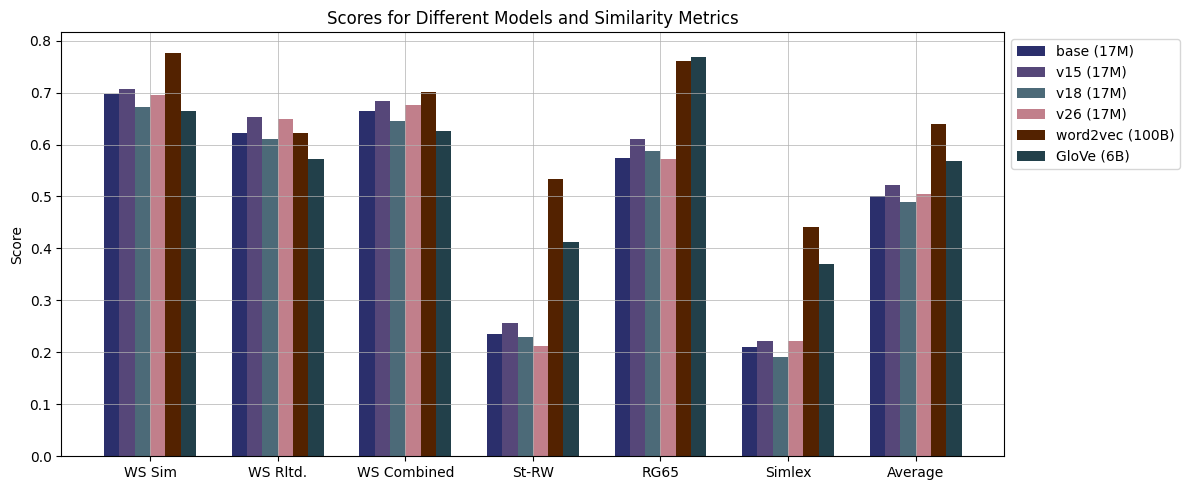
\includegraphics[width=1.0\textwidth]{img/sim_plot.png}
    \caption{Spearman rank correlation on word similarity and relatedness tasks using different benchmarks.}
    \label{fig:similarity-plot}
\end{figure}

We see that our models' performance relative to the pre-trained vectors varies greatly depending on the standard. We see that most of our models overperform GloVe on \verb|WordSim-353| similarity, and dominate both word2vec and GloVe in the relatedness. This is truly impressive, reminding you that we are comparing two pre-trained embeddings to our models that are trained on a tiny fraction of what the former were trained on. 

When we look at the other standards, however, we see a sudden change, and our models get dominated by the other two. For \verb|SimLex-999|, the accuracies are not so far off, but it proves that our model does not rank similarity over any other lexical association between words as well as other models. In the case of \verb|RW| and \verb|RG|, we reason this change merely on the corpora, given that these two benchmarks contain words that are underrepresented in our corpus. Meanwhile, other vectors are based on quite extensive datasets.

\subsubsection{Representation of similarity standards}
We now go ahead and build a base for our reasoning. For each standard, we count how many times each word appears in $V$, where $V$ is our corpora after our preprocessing step. Due to the randomness of our subsampling operation and that it mostly concerns relatively frequent words anyway, we completely disregard it. The average word occurrences for each standard, and the standard deviations of each word occurrence distribution, are given in Figure \ref{fig:occ-avg} and Figure \ref{fig:occ-dev}, respectively. 

\begin{table}[h]
  \centering
  \begin{tabular}{cc}
    \begin{subfigure}{0.47\textwidth}
      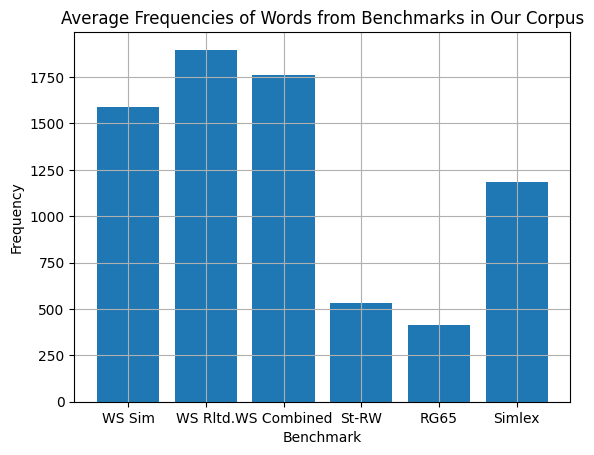
\includegraphics[width=\linewidth]{img/benchmark-occ.png}
      \caption{Average word occurrence of each benchmark}
    \label{fig:occ-avg}
    \end{subfigure} &
    \begin{subfigure}{0.47\textwidth}
      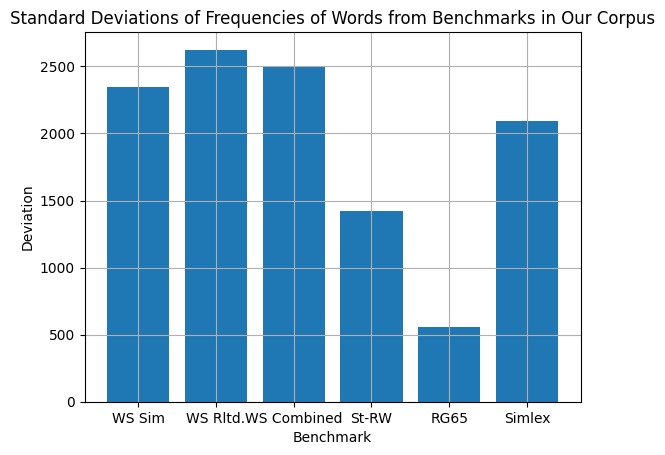
\includegraphics[width=\linewidth]{img/benchmark-std.png}
      \caption{Deviation of word occurrences of each benchmark}
    \label{fig:occ-dev}
    \end{subfigure}
  \end{tabular}
  \caption{Word occurrence statistics of each benchmark in our training corpus}
  \label{tab:occ-stats}
\end{table}

The results presented in Table \ref{tab:occ-stats} prove that the datasets we perform poorly on, except for \verb|SimLex-999|, are indeed underrepresented in our training corpus. Moreover, we see that while the words contained in \verb|WordSim-353| are represented in varying frequencies, the words in \verb|RW| and \verb|RG| are consistently underrepresented. It is unclear if the performance drop stems from this, but we believe this is a very strong factor, if not the main reason.

\subsubsection{Prediction characteristics}

We question if any of the models we use in these assessments stick to a rigid characteristic regardless of the evaluation dataset. This is clearly an undesired case, considering it would diminish the significance of this evaluation mechanism. A model that predicts more or less the same similarity for any given two words would yield good results for a dataset that contains annotations mostly in that range but would perform poorly otherwise. 

\begin{table}[ht]
\centering
\begin{tabular}{|cc|}
\hline
\multicolumn{2}{|c|}{Human Annotations} \\ \hline
\multicolumn{1}{|c|}{Predictions of the base model} & Predictions of v15 \\ \hline
\multicolumn{1}{|c|}{Predictions of v18} & Predictions of v26 \\ \hline
\multicolumn{1}{|c|}{Predictions of word2vec} & Predictions of GloVe \\ \hline
\end{tabular}
\caption{Structure of our charts}
\label{tab:str_charts}
\end{table}

We now share some histograms. We have one figure per similarity standard dataset, and each figure contains histograms of the human annotations in that dataset and the predictions made by each model. We show histograms both for our models and the pre-trained embeddings. We obtain these histograms by binning each value in one of the 10 equally divided bins in the range $[0, 10]$. To make things easier for the reader, we show the blueprint of the charts we are about to share, in Table \ref{tab:str_charts}. 

The histograms for each standard are given in Figures \ref{fig:ws_sim_table}, \ref{fig:ws_rel_table}, \ref{fig:rw_table}, \ref{fig:rg_table}, and \ref{fig:simlex_table}.

\begin{figure}[p]
    \centering
    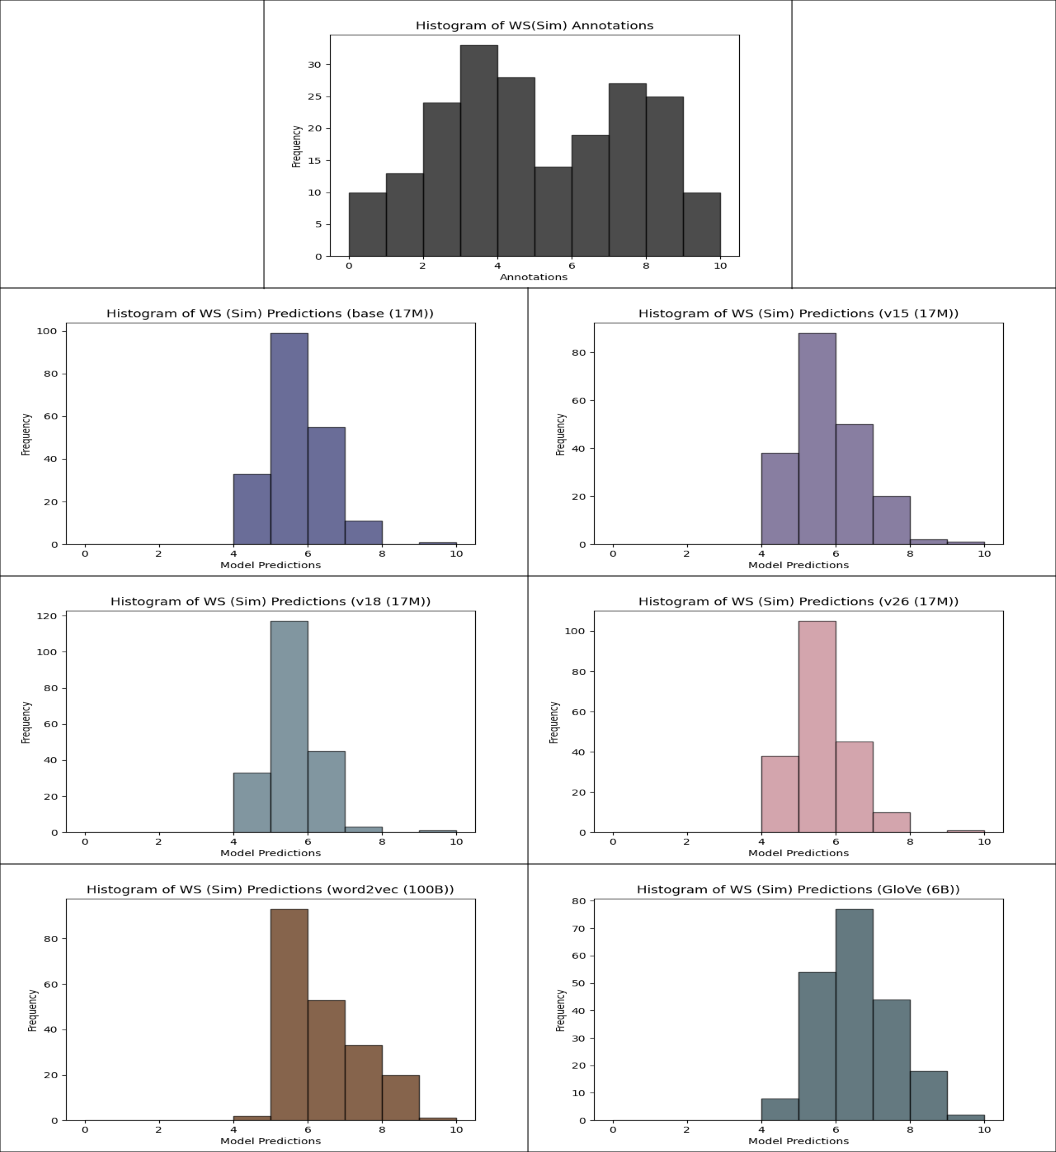
\includegraphics[width=1.0\textwidth]{img/ws_sim_table.PNG}
    \caption{Histograms for WordSim-353 Word Similarity Standard}
    \label{fig:ws_sim_table}
\end{figure}

\begin{figure}[p]
    \centering
    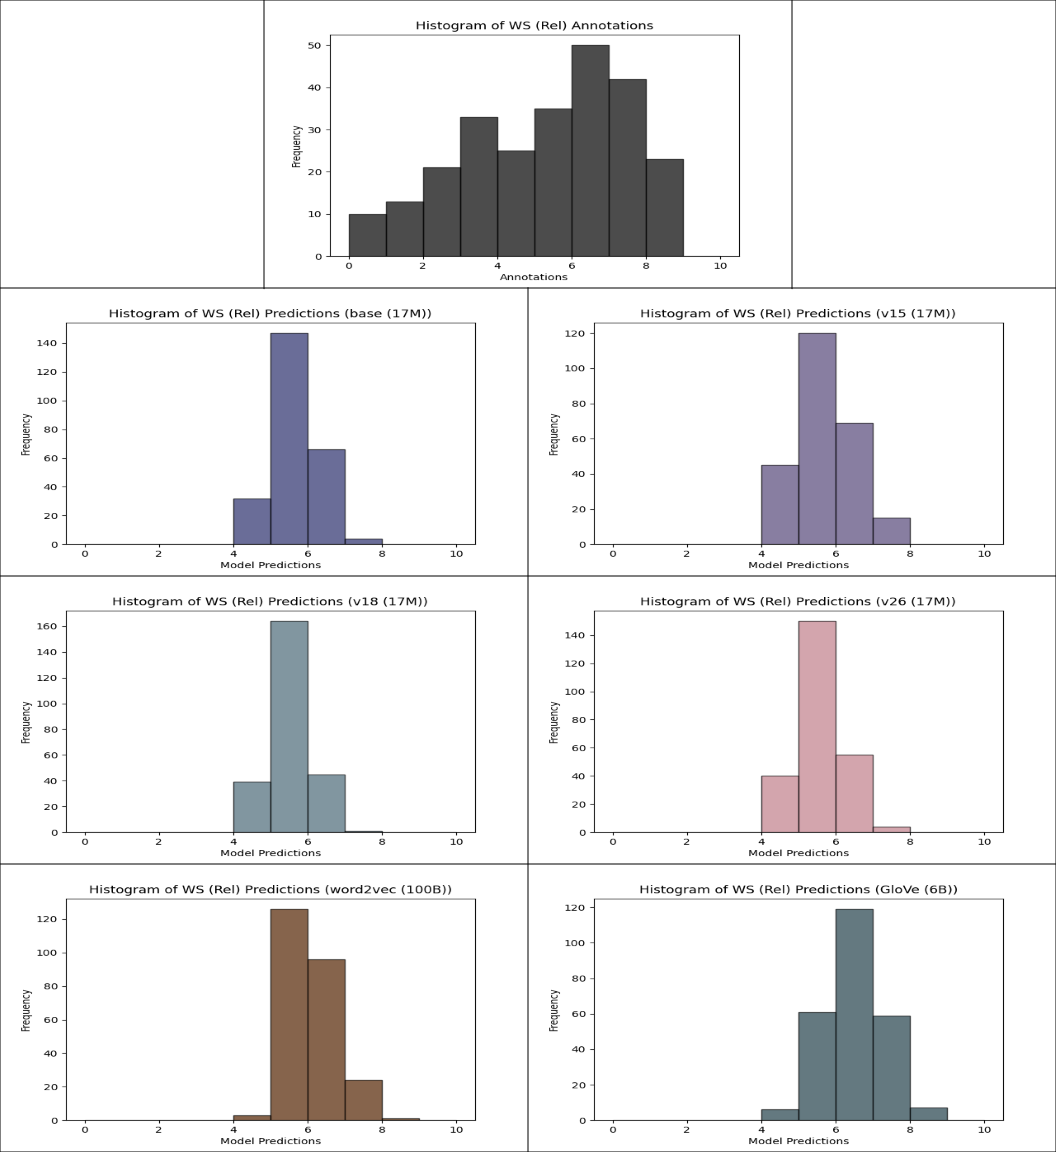
\includegraphics[width=1.0\textwidth]{img/ws_rel_table.PNG}
    \caption{Histograms for WordSim-353 Word Relatedness Standard}
    \label{fig:ws_rel_table}
\end{figure}

\begin{figure}[p]
    \centering
    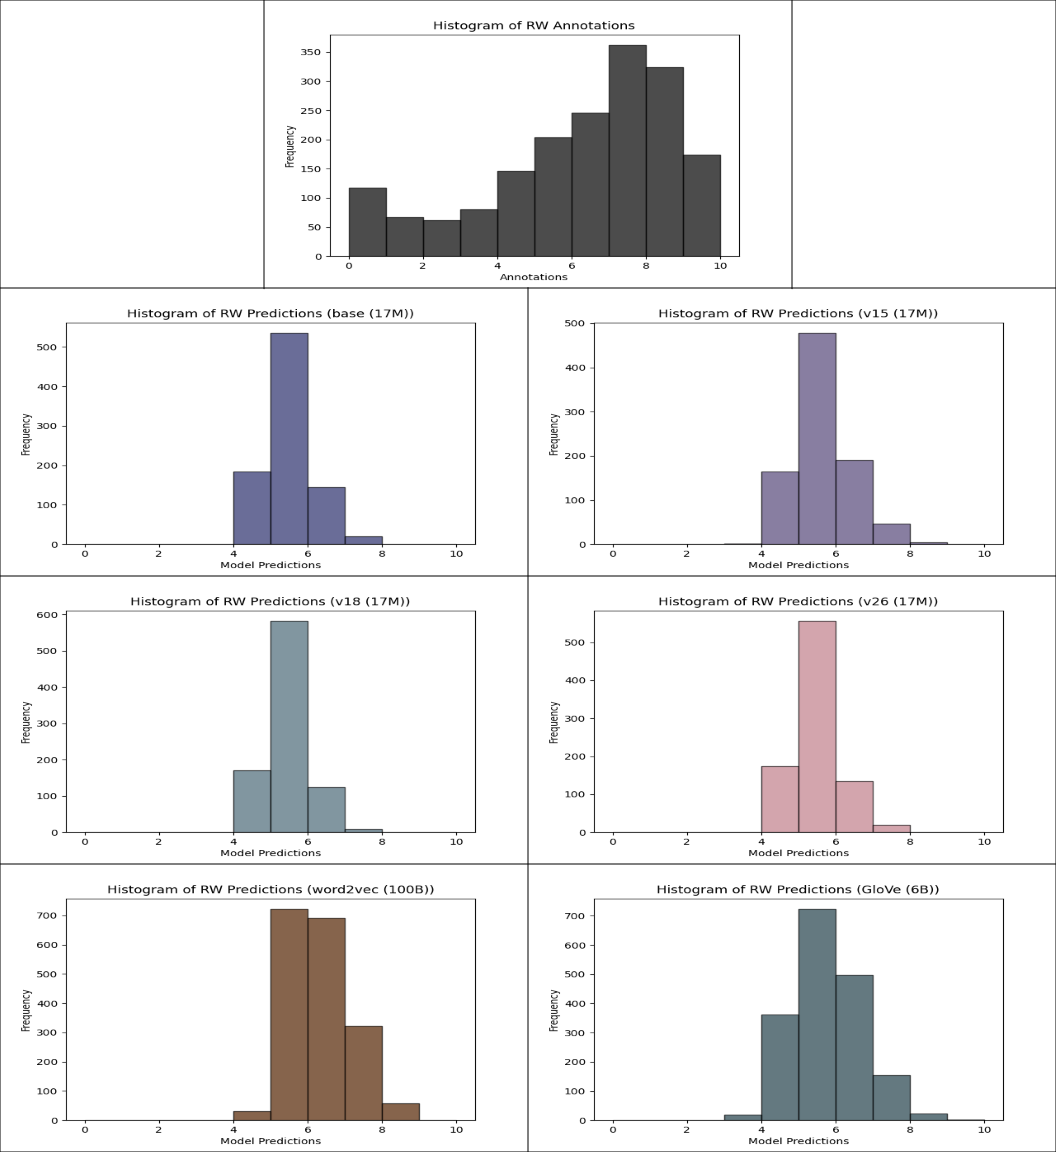
\includegraphics[width=1.0\textwidth]{img/rw_table.PNG}
    \caption{Histograms for Stanford RW Word Similarity Standard}
    \label{fig:rw_table}
\end{figure}

\begin{figure}[p]
    \centering
    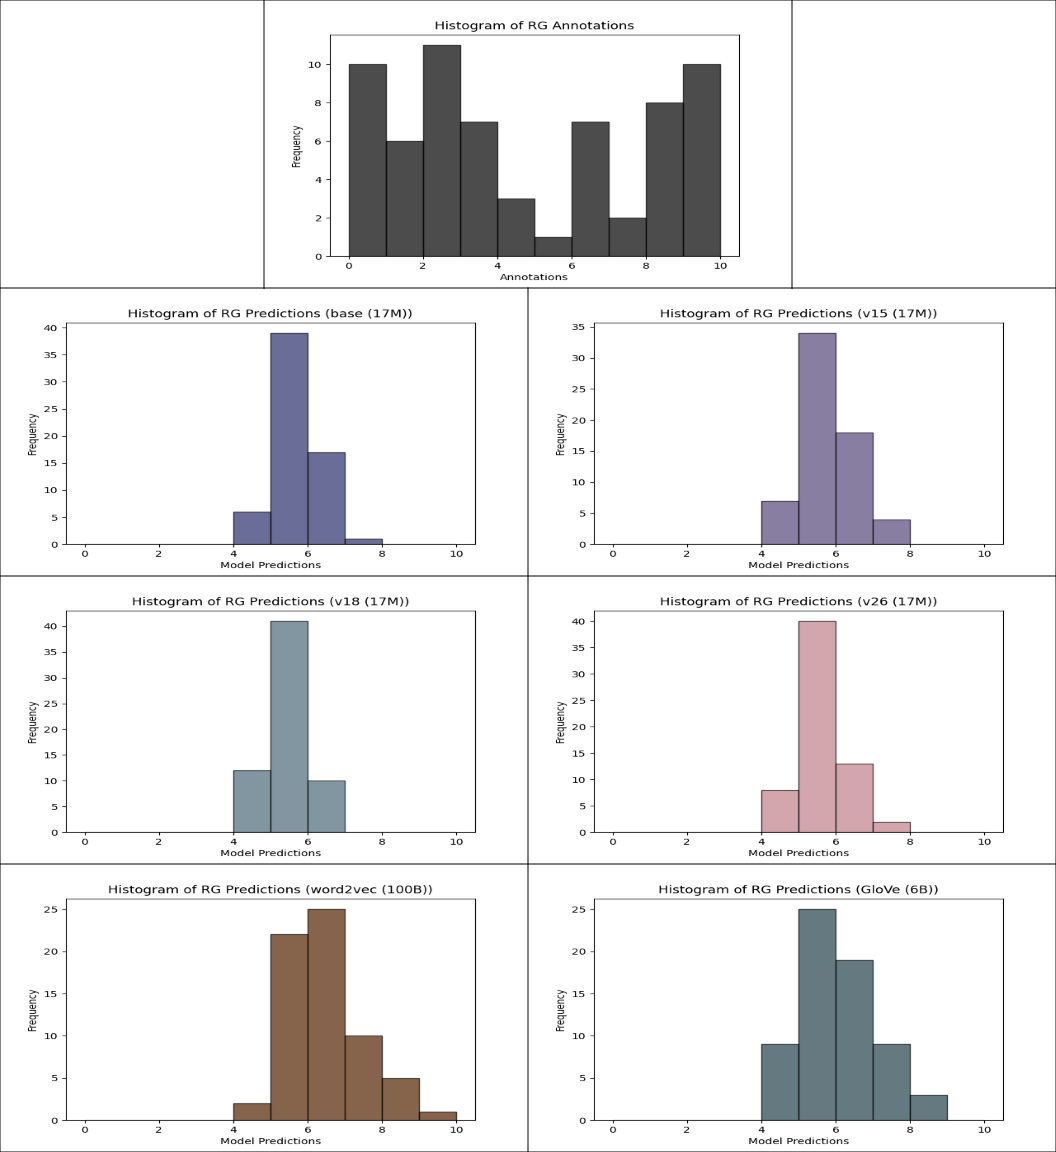
\includegraphics[width=1.0\textwidth]{img/rg_table.PNG}
    \caption{Histograms for RG-65 Word Similarity Standard}
    \label{fig:rg_table}
\end{figure}

\begin{figure}[p]
    \centering
    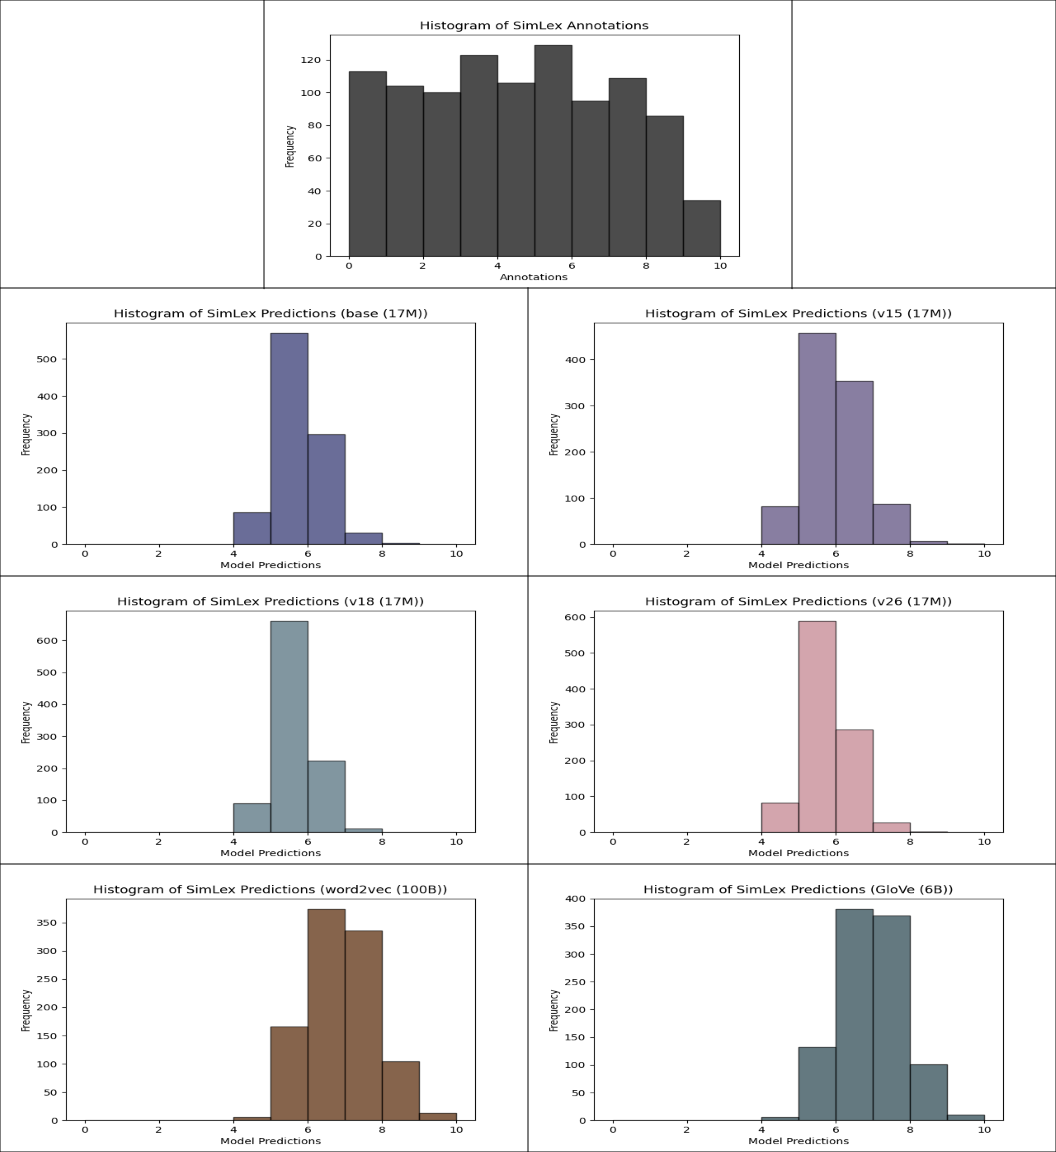
\includegraphics[width=1.0\textwidth]{img/simlex-table.PNG}
    \caption{Histograms for SimLex-999 Word Similarity Standard}
    \label{fig:simlex_table}
\end{figure}


We observe that not only the word embedding models but also the similarity standards differ from each other in terms of the ranges represented in their annotations. For example, we see somewhat of a uniform distribution in \verb|SimLex-999|, but \verb|WordSim-353| datasets favor some ranges while underrepresenting others. This issue is even more apparent in \verb|RG-65| and \verb|RW|. 

As for the models, we see that all the models almost always predict a similarity score from the range $[4, 8]$, regardless of the standard. This may not seem like a bad thing when the standard in hand is \verb|RW|, but it is certainly unideal in the case of \verb|RG-65|, considering the annotation distributions. Overall, we see that all of the models are prone to make predictions from similar ranges, resulting in similar histograms in all figures. But we also see that this issue is not bigger by a margin for our models compared to the standard ones. These findings tell us that our models do not necessarily suffer from this, but also support the points made in the article \cite{sim-problems}, which we discussed earlier in this chapter.


\subsubsection{Closer look: Some predictions}
Finally, we pick two pairs from each standard and present the predictions next to the human annotations. All values are scaled to range [0, 10], and highlight the best predictions for each sample. The results are given in Table \ref{tab:similarity_samples}.

\begin{table}[!ht]
\centering
\setlength\tabcolsep{2.5pt}
\begin{tabular}{|ccc|cccc|cc|}
\hline
\textbf{Pair} & \textbf{Standard} & \textbf{Score} & \textbf{base} & \textbf{v15} & \textbf{v18} & \textbf{v26} & \textbf{w2v} & \textbf{GloVe} \\ \hline
\textit{tiger, cat} & WS (Sim) & 7.35 & \underline {6.27} & 6.18 & 5.64 & 5.59 & \textbf{7.59} & 6.56 \\
\textit{king, cabbage} & WS (Sim) & 0.23 & 4.66 & 4.42 & 4.55 & \underline {\textbf{4.31}} & 5.59 & 4.93 \\
\textit{day, summer} & WS (Rel) & 3.94 & 5.76 & 5.93 & \underline {\textbf{5.46}} & 5.75 & 7.24 & 7.38 \\
\textit{professor, cucumber} & WS (Rel) & 0.31 & 4.79 & 4.80 & \underline {\textbf{4.27}} & 4.48 & 5.28 & 4.73 \\
\textit{imperfection, state} & RW & 0.29 & 5.21 & 5.03 & 5.08 & \underline {4.92} & 5.27 & \textbf{4.41} \\
\textit{friendships, brotherhood} & RW & 7.50 & 5.63 & \underline {5.88} & 5.36 & 5.58 & \textbf{7.32} & 5.87 \\
\textit{cord, smile} & RG-65 & 0.05 & 5.00 & 5.54 & \underline {\textbf{4.79}} & 5.21 & 5.09 & 5.37 \\
\textit{gem, jewel} & RG-65 & 9.85 & 5.59 & \underline {6.02} & 5.22 & 5.61 & \textbf{8.11} & 7.41 \\
\textit{smart, intelligent} & SimLex & 9.20 & 5.27 & 5.14 & 5.08 & \underline {5.94} & 8.25 & \textbf{8.26} \\
\textit{hard, easy} & SimLex & 0.95 & 6.13 & 6.23 & \underline {\textbf{5.75}} & 5.97 & 7.36 & 7.89 \\ \hline
\end{tabular}
\caption{Similarity scores of some word pairs selected from standard datasets and predictions of each model. All scores are scaled to range {[}0, 10{]}. Bold indicates the best estimate of all predictions, and underline indicates the best estimate among our models.}
\label{tab:similarity_samples}
\end{table}

\subsection{Results: Word analogy}

Even though since the very beginning of our study, we did not put any emphasis on the word analogy tasks, we still acknowledge that it is yet another important type of assessment of the quality of static word embeddings in terms of capturing lexical contextual relationships. Unlike our way of thinking, studies like \cite{glove} and \cite{w2v} focus more on the analogy tasks than any other in terms of evaluation techniques. As we described earlier, we built an evaluation process for this task identical to what is considered standard in the literature and also added another version by replacing cosine similarity with Euclidean distance. We show how our models compare to others in both of these versions, in Table \ref{tab:analogy-table}. Then these results are visualized in Figure \ref{fig:analogy-plot}. 

\begin{table}[h]
\centering
\setlength\tabcolsep{4pt}
\begin{tabular}{|ccc|cc|}
\hline
Model & Dimension & Size & Cosine Similarity Based & Euclidean Based \\ \hline
base & 300 & 17M & 0.12 & 0.03 \\
v15 & 300 & 17M & 0.15 & 0.06 \\
v18 & 300 & 17M & 0.06 & 0.01 \\
v26 & 300 & 17M & 0.11 & 0.02 \\ \hline
GloVe & 300 & 6B & \textbf{0.72} & \textbf{0.70} \\
word2vec & 300 & 100B & 0.54 & 0.48 \\ \hline
\end{tabular}
\caption{Accuracies on two versions of the word analogy task}
\label{tab:analogy-table}
\end{table}

\begin{figure}[h]
    \centering
    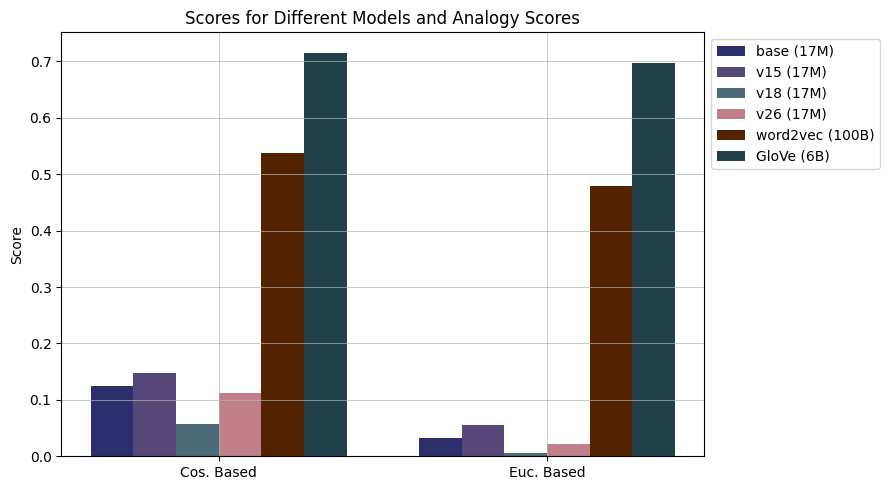
\includegraphics[width=0.8\textwidth]{img/analogy-plot.png}
    \caption{Accuracies on two versions of the word analogy task}
    \label{fig:analogy-plot}
\end{figure}

We observe that our models come nowhere near the standard models in this particular task. We also observe the impressive accuracy achieved by GloVe, demonstrating its versatility, surpassing the word2vec model which is based on a larger corpus by a wide margin. It is difficult to tell how can we reasonably interpret these results, but the following are our estimates of what this poor performance might be stemming from.

\begin{itemize}
    \item \textbf{Validity}: Even though we followed exactly how this task is described in the literature, there is still no solid proof that this is the best way to reveal a word embedding model's abilities. There are several studies in the literature, such as \cite{analogy1} and \cite{analogy2}, criticizing both this way of implementation and the validity of this task altogether. Therefore we suspect the suitability of our models to this way of calculation of word analogy accuracy, but this is a topic to investigate in a follow-up study.
    \item \textbf{The effect of model selection}: In each study for developing a static word embedding model, or any sort of machine learning model, the final version to be presented is selected based on some sort of performance metric. This metric is to comparatively evaluate the performance of a model and the other versions developed in the course of that study. In our case, our emphasis was on the word similarity-based evaluations. Judging from their publications, we suspect that the model selection in other models' developments might be based on word analogy instead. However, even if this is true, it is difficult to argue that this would cause this big of a performance difference. 
    \item \textbf{Suitability}: What makes a word embedding model good at word analogies, or what could cause a model to be bad at it, are questions that are out of the scope of our study. But without any proof that supports our other hypothesis, we can simply assume that our model is not suitable for this task. Therefore we should either admit that there is a lot of room for improvement or not use this metric to assess the quality of our vectors at all.
\end{itemize}

\subsection{Results: Word Sense Distinction}

Dealing with different word senses is not usually a performance indicator for static word embeddings. Static word embeddings, like word2vec or GloVe, are very limited when it comes to handling different senses of words. Static embedding models learn a single vector representation for each type, regardless of context or sense. As a result, they tend to mix up the various senses of a word into a single representation. This is the reason we usually go with dynamic embeddings if the downstream \ac{NLP} task requires a distinction of word senses. Nevertheless, with our custom word sense distinction task, we are looking if it is possible to deal with different word senses using static word embeddings. The results (scaled by 100) are given in Table \ref{tab:word-sense-tab}. The results are visualized for a clearer comparison in Figure \ref{fig:sense-plot}.

\begin{table}[h]
\centering
\begin{tabular}{|ccc|cc|}
\hline
Model & Dimension & Size & Projection Based & Cosine Similarity Based \\ \hline
base & 300 & 17M & 1.67 & 1.58 \\
v15 & 300 & 17M & 2.09 & 1.93 \\
v18 & 300 & 17M & 2.14 & 2.04 \\
v26 & 300 & 17M & 1.22 & 1.23 \\ \hline
GloVe & 300 & 6B & 0.8 & -0.15 \\
word2vec & 300 & 100B & -0.03 & -0.89 \\ \hline
\end{tabular}
\caption{Results of the word sense distinction task (Scaled by 100)}
\label{tab:word-sense-tab}
\end{table}

\begin{figure}[h]
    \centering
    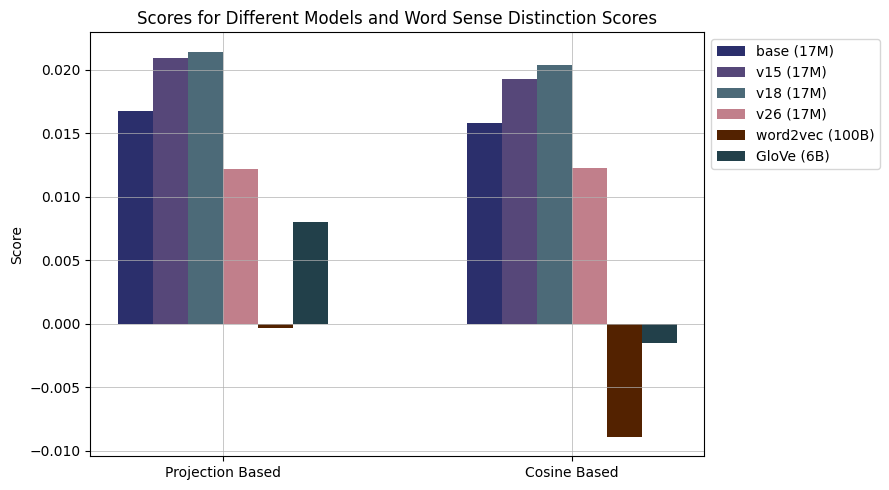
\includegraphics[width=0.9\textwidth]{img/sense-plot.png}
    \caption{Results of the word sense distinction task}
    \label{fig:sense-plot}
\end{figure}

The first observation to make is that our models provide positive valued scores, which is what we were hoping for. The challenge with this metric is that we can only estimate the score that would indicate success, considering that this is a custom process and we do not have a standard for it. Therefore we will consider any positive score as a good indication. 

Secondly, we see that our models dominate the pre-trained ones by a margin. This is also what we were hoping for, but also what we were expecting. We see that according to this metric, the pre-trained models have no ability to tell apart different word senses, while we have this ability in our embeddings.

Thirdly, we see that version 26, which is the one that omits the positive loss $\myscore{+}{w, u_1, u_2}$ from its loss, is our weakest model. We understand the impact of $\myscore{+}{w, u_1, u_2}$ in word sense distinction from this observation. This is perhaps the most valuable observation we made in this experiment since it finally provides a hint about the existence of the context hyperplanes, which we so far failed to prove their existence.

We should note again that this is a fully custom process, which is supported by a fully custom dataset. The evaluation task is not thought in depth as much as other standard evaluation techniques in the literature. Its performance indicator does not have a standard comparison and can be improved to be easier to understand. The dataset is a toy dataset at its best compared to datasets like \verb|SimLex-999|, which is produced by 500 human annotators who are native in English \cite{simlex}. However, we still believe these results are meaningful for showing the sense distinction abilities of our models, especially considering that we did not use this evaluation technique in our model selection procedure.

\newpage

\section{Exploring the effects of training data size on model performance}
\label{sec:data_size}

We mentioned before that it is impressive that our model is comparable to other pre-trained embeddings in some metrics, and we mainly based this on the dramatic difference in the size of the training data. However, in order to claim this, we are very much aware that we need to provide some sort of base by proving that the quality of our embeddings is proportional to the size of the training data we used. 

In this section, we will do exactly that, and investigate the influence of training corpus size on our model's performance. We will share the achieved accuracies of different versions of our base model on different evaluation tasks. These versions differ from each other in terms of the training data we use to train them. We systematically trained our base model using 12.5\%, 25\%, 50\%, and 100\% of our training corpus, maintaining consistent data quality and preprocessing methods across all subsets. 

Instead of slicing a portion of the data and using it, we partitioned the entire corpus into 128 bins and joined the required number of bins by picking them in intervals. This way, we tried to keep the representations of words relative to the size of the dataset somewhat the same.

\subsection{Similarity and relatedness}

Table \ref{tab:sim-scale} shows how the accuracy in word similarity/relatedness evaluations changes with the scale of the training data. Our findings in this test align with expectations, revealing a clear relation between the size of the training data and the model's similarity-based evaluation performance. We then visualize these findings in Figure \ref{fig:sim-scale}.

\begin{table}[h]
\centering
\setlength\tabcolsep{3pt}
\begin{tabular}{|ccc|cccccc|}
\hline
Model & Dimension & Portion & WS (Sim) & WS (Rel) & WS (Avg) & RW & RG & SimLex \\ \hline
base & 300 & 12.5\% & 0.29 & 0.33 & 0.31 & 0.03 & 0.20 & 0.11 \\
base & 300 & 25\% & 0.56 & 0.47 & 0.52 & 0.17 & 0.46 & 0.15 \\
base & 300 & 50\% & 0.61 & 0.59 & 0.60 & 0.19 & 0.49 & 0.17 \\
base & 300 & 100\% & \textbf{0.70} & \textbf{0.62} & \textbf{0.66} & \textbf{0.24} & \textbf{0.57} & \textbf{0.21} \\ \hline
\end{tabular}
\caption{Results of the word similarity/relatedness task, using increasing scales of the corpus}
\label{tab:sim-scale}
\end{table}

\begin{figure}[h]
    \centering
    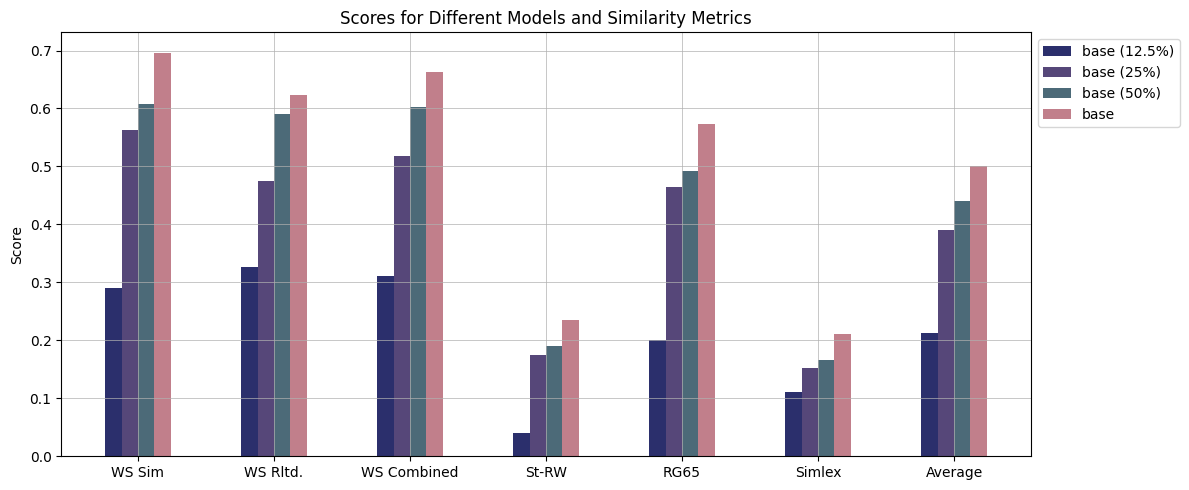
\includegraphics[width=0.9\textwidth]{img/sim-scale.png}
    \caption{Results of the word similarity/relatedness task, using increasing scales of the corpus}
    \label{fig:sim-scale}
\end{figure}


\subsection{Word analogy}

We now do the same for the word analogy task and put our different-sized models head to head for the word analogy task, and provide the results. Accuracies of our models are provided in Table \ref{tab:analogy_scale}. In Figure \ref{fig:analogy_scale}, we visualize these results for a clear comparison.

\begin{table}[h]
\centering
\begin{tabular}{|ccc|cc|}
\hline
Model & Dimension & Portion & Cosine Similarity Based & Euclidean Based \\ \hline
base & 300 & 12.5\% & 0.009 & 0.008 \\
base & 300 & 25\% & 0.038 & 0.022 \\
base & 300 & 50\% & 0.053 & 0.015 \\
base & 300 & 100\% & \textbf{0.125} & \textbf{0.032} \\ \hline
\end{tabular}
\caption{Results of the word analogy task, using increasing scales of the corpus}
\label{tab:analogy_scale}
\end{table}


\begin{figure}[h]
    \centering
    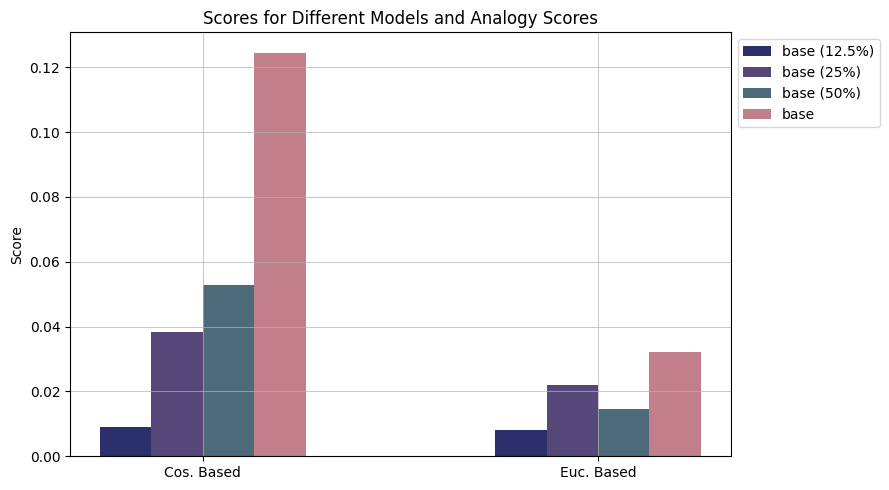
\includegraphics[width=0.7\textwidth]{img/analogy_scale.png}
    \caption{Results of the word analogy task, using increasing scales of the corpus}
    \label{fig:analogy_scale}
\end{figure}

Except for one incident we observe in the Euclidean-based metric, we see a direct relation between the corpus size and the model accuracy in the word analogy task, proving that as the training data gets larger, our models capture lexical relationships with a better performance.


\subsection{Word Sense Distinction}

Finally, we provide our observations in the word sense distinction set, in Table \ref{tab:sense_scale} (scaled by 100). We visualize these scores in Figure \ref{fig:sense_scale}.

\begin{table}[h]
\centering
\begin{tabular}{|ccc|cc|}
\hline
Model & Dimension & Portion & Projection Based & Cosine Similarity Based \\ \hline
base & 300 & 12.5\% & 0.55 & 0.58 \\
base & 300 & 25\% & \textbf{2.22} & \textbf{2.20} \\
base & 300 & 50\% & 1.92 & 1.70 \\
base & 300 & 100\% & 1.67 & 1.58 \\ \hline
\end{tabular}
\caption{Results of the word sense distinction task, using increasing scales of the corpus (Scaled by 100)}
\label{tab:sense_scale}
\end{table}

\begin{figure}[h]
    \centering
    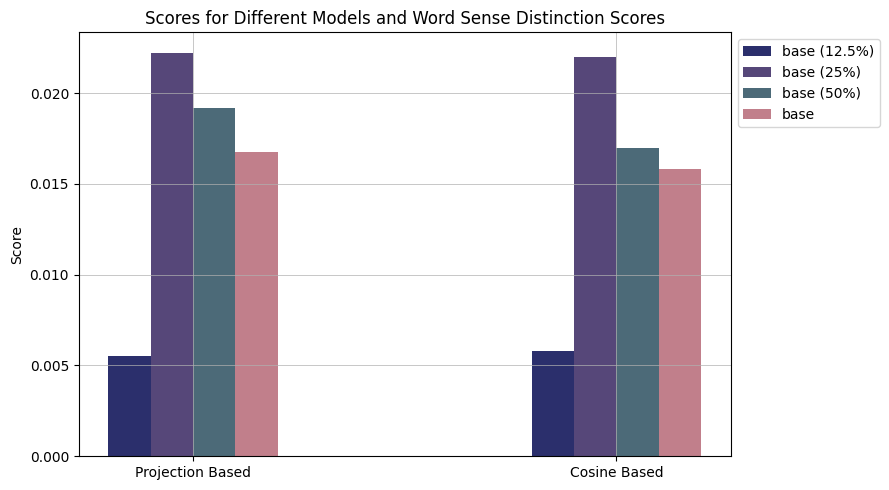
\includegraphics[width=0.7\textwidth]{img/sense_scale.png}
    \caption{Results of the word sense distinction task, using increasing scales of the corpus}
    \label{fig:sense_scale}
\end{figure}

This is the only task in which we do not observe a proportion between the dataset size and the model performance. Interestingly, the relation is not inverse either. The best performance seems to be achieved by the model with 25\% in size, and the worst one is the smallest model with 12.5\% in size.

Combining all these observations, apart from the latest one, all of our experiments give us a clear indication of the performance boost relative to the dataset size. Based on these, we find the courage to claim that our model has the potential to achieve much better results, surpassing the standard models in some cases and competing with them in others, when a similar amount of training data is provided.



\section{Analyzing the impact of noise word positioning on model consistency}

So far, all of our models aimed to push the noise projections to the left side of the context projections along the target vector. This seemed to achieve satisfactory results, but now we are curious whether or not we can achieve similar results or better, when we do the opposite and push the noise projections to the right instead.

To investigate this, we kept everything the same but altered just one thing in our base model, so that we obtain this new behavior from the same architecture. The only thing that is changed compared to the original base model is the calculation of the projection difference $D$. Using the same notation as Section \ref{sec:neg_loss}, $D$ is now calculated as:

\[ 
D = \frac{e_c(u_3) \cdot e_t(w) - e_c(u_1) \cdot e_t(w)}{\left \| e_t(w) \right \|}
\]

We refer to this new model as \textbf{version 27}. To make sure we get exactly the behavior we desire, we calculated some statistics using this new model. These are the same statistics we calculated for our top-performing models, therefore the interpretation and the comparison will be fairly straightforward.

\begin{figure}[h]
    \centering
    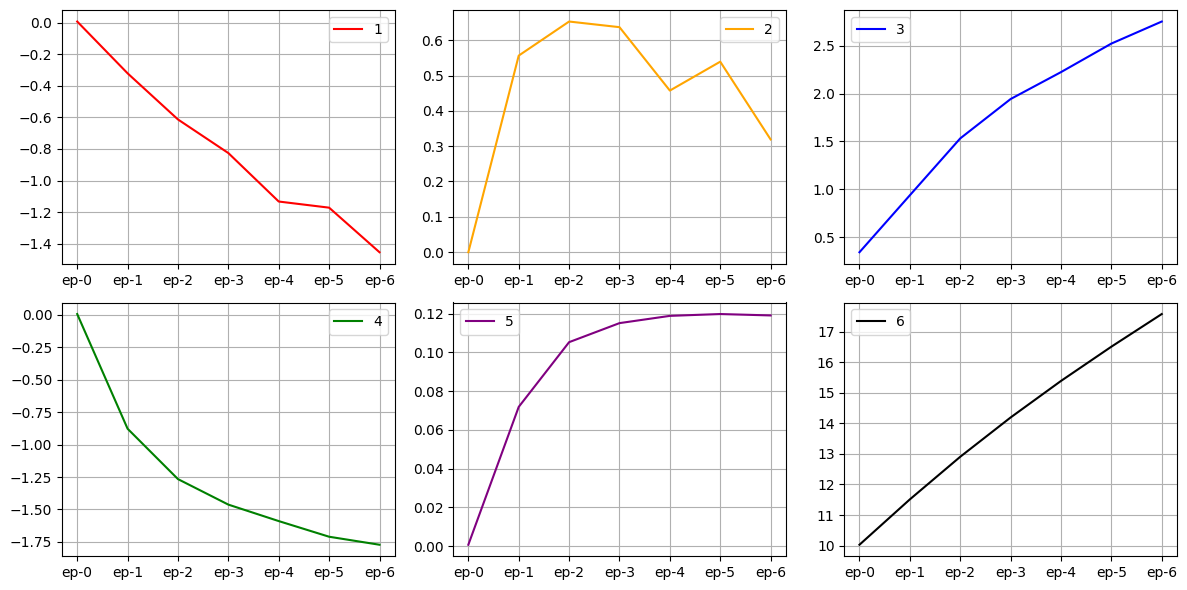
\includegraphics[width=0.9\textwidth]{img/pushleft-stats.png}
    \caption{Statistics computed for the model version 27}
    \label{fig:pushleft-stats}
\end{figure}

Figure \ref{fig:pushleft-stats} shows the statistics computed for this new model. The statistics visualized here are exactly the same ones as in Section \ref{sec:stats}, therefore the reader is advised to refer to that section for the descriptions of these statistics. Opposite of the other models we presented earlier, now we see that as the training proceeds, our context projections get shorter, while the noise projections get longer, at least up to some point. Subsequently, statistic \#4 seems to go down consistently as the learning proceeds, the exact opposite of what we see in the other models. This proves that the desired behavior is obtained. 

\begin{figure}[h]
    \centering
    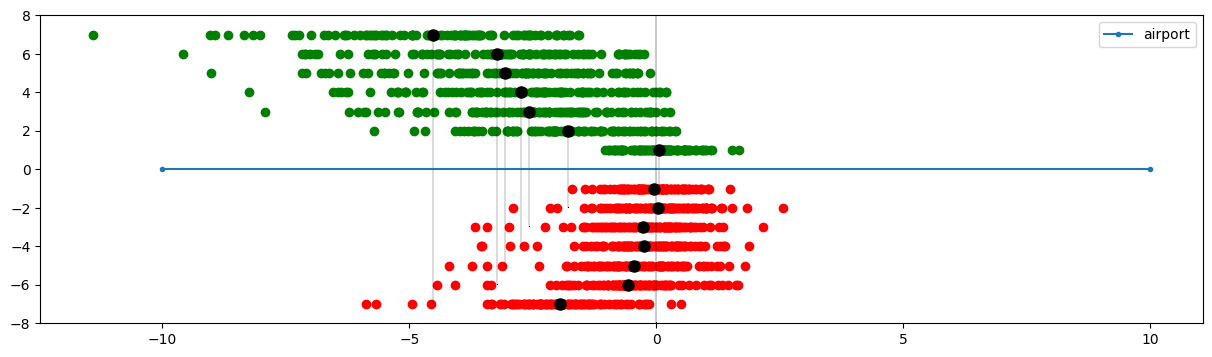
\includegraphics[width=0.9\textwidth]{img/airport_left.png}
    \caption{For the target word "airport", vector projections in different epochs, using the model version 27}
    \label{fig:airport_left}
\end{figure}

To make things more visual, we show how vector projections change as the training loop iterates, in Figure \ref{fig:airport_left}. This figure is similar to the figures presented in Section \ref{sec:vis_proj}, therefore the reader is advised to go through the descriptions provided there. As for the model performance, we conducted the same evaluations as described in Section \ref{sec:tasks_datasets} on this new model and compared it to the original base model. The exact scores are omitted as they are not so relevant now, and we show the graphs comparing these two models only instead.

\begin{table}[p]
  \centering
  \begin{tabular}{cc}
    \begin{subfigure}{0.9\textwidth}
      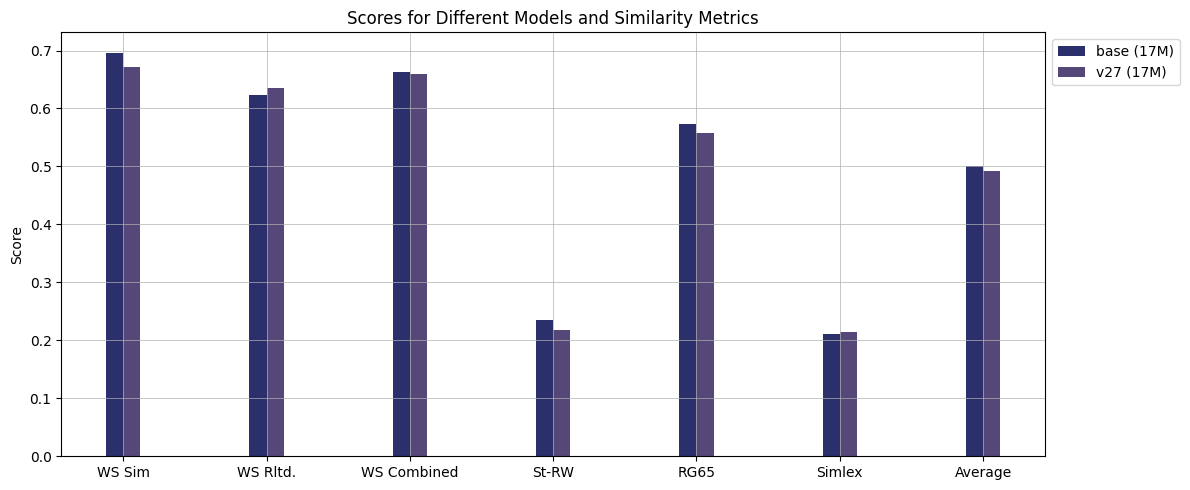
\includegraphics[width=\linewidth]{img/sim_v27.png}
      \caption{Word similarity \& relatedness tasks, base model versus version 27}
    \end{subfigure} \\
    \begin{subfigure}{0.8\textwidth}
      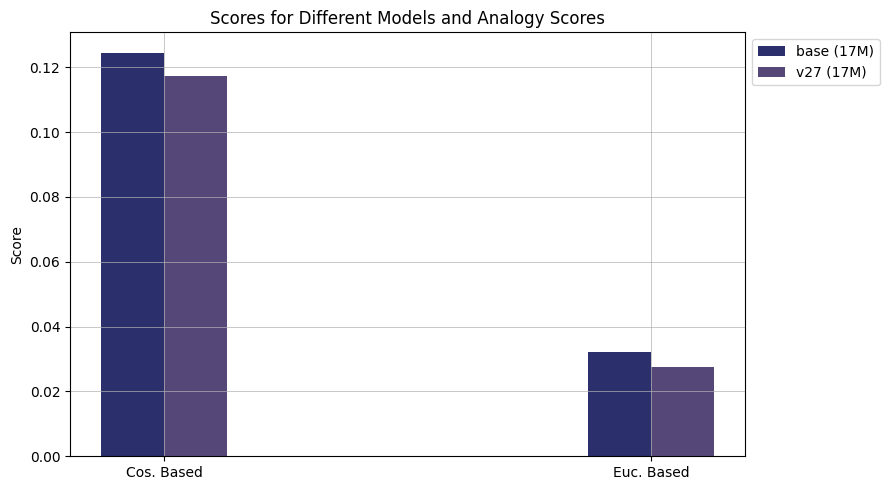
\includegraphics[width=\linewidth]{img/analogy_v27.png}
      \caption{Word analogy task, base model versus version 27}
    \end{subfigure} \\
    \begin{subfigure}{0.8\textwidth}
      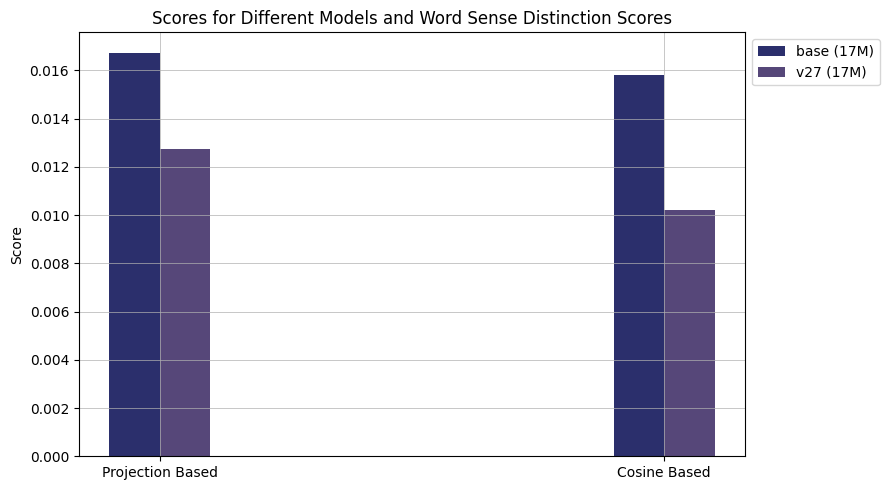
\includegraphics[width=\linewidth]{img/wsd_v27.png}
      \caption{Word sense distinction task, base model versus version 27}
    \end{subfigure}
  \end{tabular}
  \caption{Evaluations conducted on the model version 27, compared to the base model}
  \label{tab:basev27}
\end{table}

Table \ref{tab:basev27} shows the performance of this new model, version 27, on our set of evaluation tasks, and how it compares to what is achieved in the base version.

These results show that version 27 is almost never able to achieve the exact scores achieved by the base model, but we are fairly close. For the purpose of this section, the latter part is more important for us. We can now say that as long as we separate noise and context projections onto the target vector, our models are able to achieve somewhat similar results, regardless of the direction chosen.



% $\myscore{+}{w, u_1, u_2}$

